% !TEX root = ../notes_template.tex
\chapter{Spatial Models} \label{sec:Chap5}

\section{Exogenous and Endogenous Drivers of Spatial Patterns}
Ecologists often seek to identify the processes that underlie patterns that they observe in nature.  For example, community ecologists have classified vegetation communities based on local temperature and precipitation, and subsequently identified tradeoffs in plant structure and metabolic constraints that underlie these \cite{ricklefs_economy_2008}.  In this case, an ecologist might construct a regression predicting vegetation densities as a function of local precipitation and temperature, and might seek to develop a statistical model that explains a large portion of observed variance.  As another example, meta-population theory arose from describing how butterfly movement between habitat patches can ``rescue" local extirpation arising from small population sizes in each individual patch \cite{hanski_checkerspots_2004}.  In this latter case, the variable of interest (abundance in each habitat patch) is expected to vary stochastically (due to low sample sizes for individual birth and death) such that environmental covariates are not sufficient in isolation to explain demographic variation.  

These two examples illustrate that spatial patterns arise both from:
\begin{itemize}
    \item \textit{Exogenous drivers}, i.e., where physical habitat constraints (e.g., temperature and precipitation) drive population densities via their effect on demographics (birth, death, growth, movement, etc.);

    \item \textit{Endogenous drivers}, i.e., where age-structured movement, density-dependent habitat selection, selective social information usage \cite{loukola_observed_2013}, and other properties of a given population or community might cause a particular form of spatial aggregation to arise. 
\end{itemize}
This distinction becomes important because analysts might hope to eventually identify and measure the exogenous drivers that are associated with spatial variation in population density.  However, even in this perfect world where all exogenous drivers have been identified and measured, there will always be endogenous drivers of spatial distribution that cause local densities to not reflect long-term averages.  

When endogenous drivers have a large role, or when important exogenous drivers have not been measured, regressing population density on available covariates is likely to result in large residuals (i.e., instances where observations are much larger or smaller than model predictions), where these residuals are then correlated for nearby samples.  Neglecting these spatially correlated residuals will cause predicted densities to be a poor description of underlying patterns, and therefore cause any downstream ecological interpretation to be suspect.  

In practice, ecologists generally recognize the importance of accounting for residual patterns that are correlated across space, time, or among variables (e.g., between ages, species, etc.), both when fitting models \cite{dormann_correlation_2012} and when evaluating their performance \cite{roberts_cross-validation_2017}.  Ecologists have therefore developed a wide range of techniques to account for residuals spatial variation \cite{dormann_collinearity_2013}.  In the following chapter, we contrast widely used methods to estimate spatially correlated residual patterns, while emphasizing those that can combined with other types of ecological dynamics in later chapters.    

\section{Basis Expansion and Splines} \label{sec:Chap5:splines}

In Section \ref{sec:Chap1_GLM}, we introduced Generalized Linear Models (GLMs), which we described as a model having a linear predictor \( \mu_i \), link function \(g\), and probability distribution \(f\) defining the likelihood of data given parameters:

\begin{gather}
    Y_i \sim f(\mu_i) \\
    g(\mu_i) = \mathbf{x}_i \mathbf{\beta}
\end{gather}
We first focus on approaches that address residual spatial variation by increasing the flexibility of available covariates\footnote{See https://github.com/james-thorson/Spatio-temporal-models-for-ecologists/Chap\_5 for code associated with this chapter.}.  

To define model ``flexibility" we first introduce the concept of \myindex{degrees of freedom}, which measures the the number of dimensions that are necessary to describe the predictions from a model.  For example, consider a model where covariate matrix \( \mathbf X \) includes a column of \(1s\) (representing an intercept) and then a single covariate.  In this case, there's (at most) two degrees of freedom for the predicted density surface \( \mathbf{\mu = X \beta} \), represented by the vector of coefficients \( \mathbf{\beta} \) (Fig. \ref{fig:Chap5_Basis_linear}).  Put another way, the potential  densities \( \mu \) could be described as the sum of two \textit{basis functions}.  To increase model flexibility, we could therefore expand the number of basis functions that are needed to describe the predicted response \( \mu \).  

\begin{figure}[!ht]
    \caption[Linear model basis functions]{Illustration of the basis functions resulting from a single intercept and covariate (top panel) representing elevation in km in China, and ten random simulations of the density function that could arise from using this basis (bottom panel).}
    \centering
    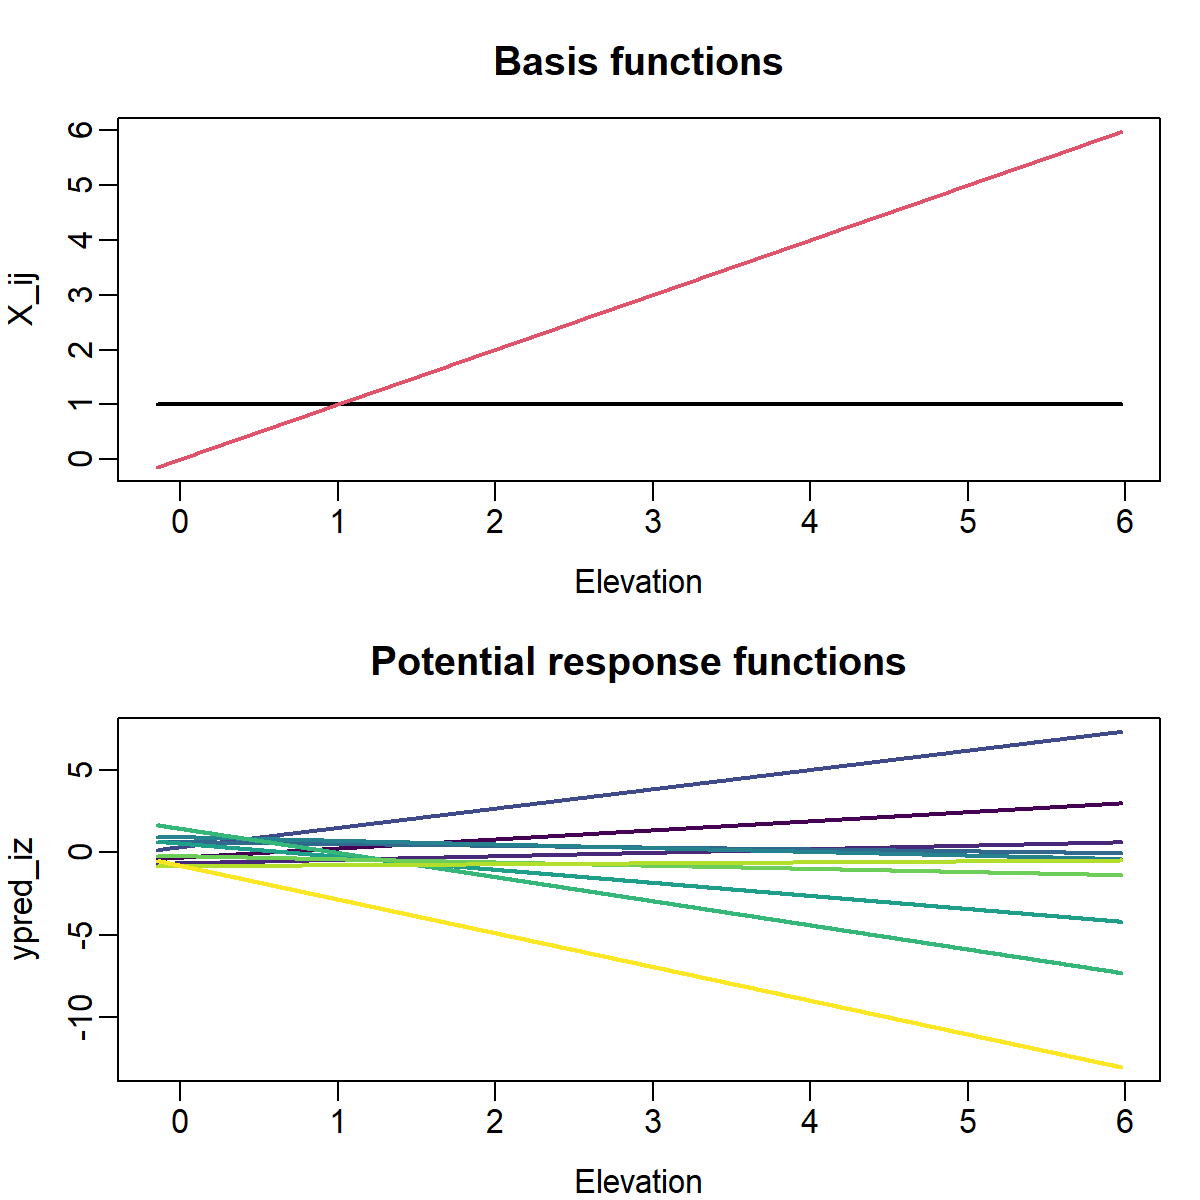
\includegraphics[width=4in]{Chap_5/Basis-linear.png}
    \label{fig:Chap5_Basis_linear}
\end{figure}

To increase the flexibility of this GLM, we therefore apply \myindex{basis expansion} to create an expanded set of covariates \( \mathbf{X}^* \), and an associated increase in the degrees of freedom \( \mathbf{\beta} \).  Basis expansion involves specifying a function \(b : X \mapsto \mathbf X^*\) that transforms the original covariates \(\mathbf{X}\) to an expanded set of covariates \(\mathbf{X}^*\) where the rank of \( \mathbf X^*\) is greater than that of \( \mathbf{X}\).  In practice, basis expansion often takes as input one or two covariate vectors, and as output gives an expanded set of covariate vectors.  The simplest example is quadratic expansion, where a covariate vector (e.g., elevation) is replaced with two vectors, representing elevation and elevation-squared (Fig. \ref{fig:Chap5_Basis_polynomial}).  This then allows the potential response function \( \mathbf{X^* \beta} \) to generate a dome-shaped response, potentially identifying the value of a given covariate where densities are expected to be highest.  Quadratic basis expansion is one example of polynomial basis expansion, where a covariate \(X\) is combined with its polynomials, e.g., its square \(X^2\), cube \(X^3\), etc.   

\begin{figure}[!ht]
    \caption[Basis functions using 2nd-order polynomial basis expansion]{Illustration of the basis functions resulting from a single intercept and covariate (top panel) that is transformed using a quadratic polynomial basis expansion, and ten random simulations of the density function that could arise from using this basis (bottom panel).}
    \centering
    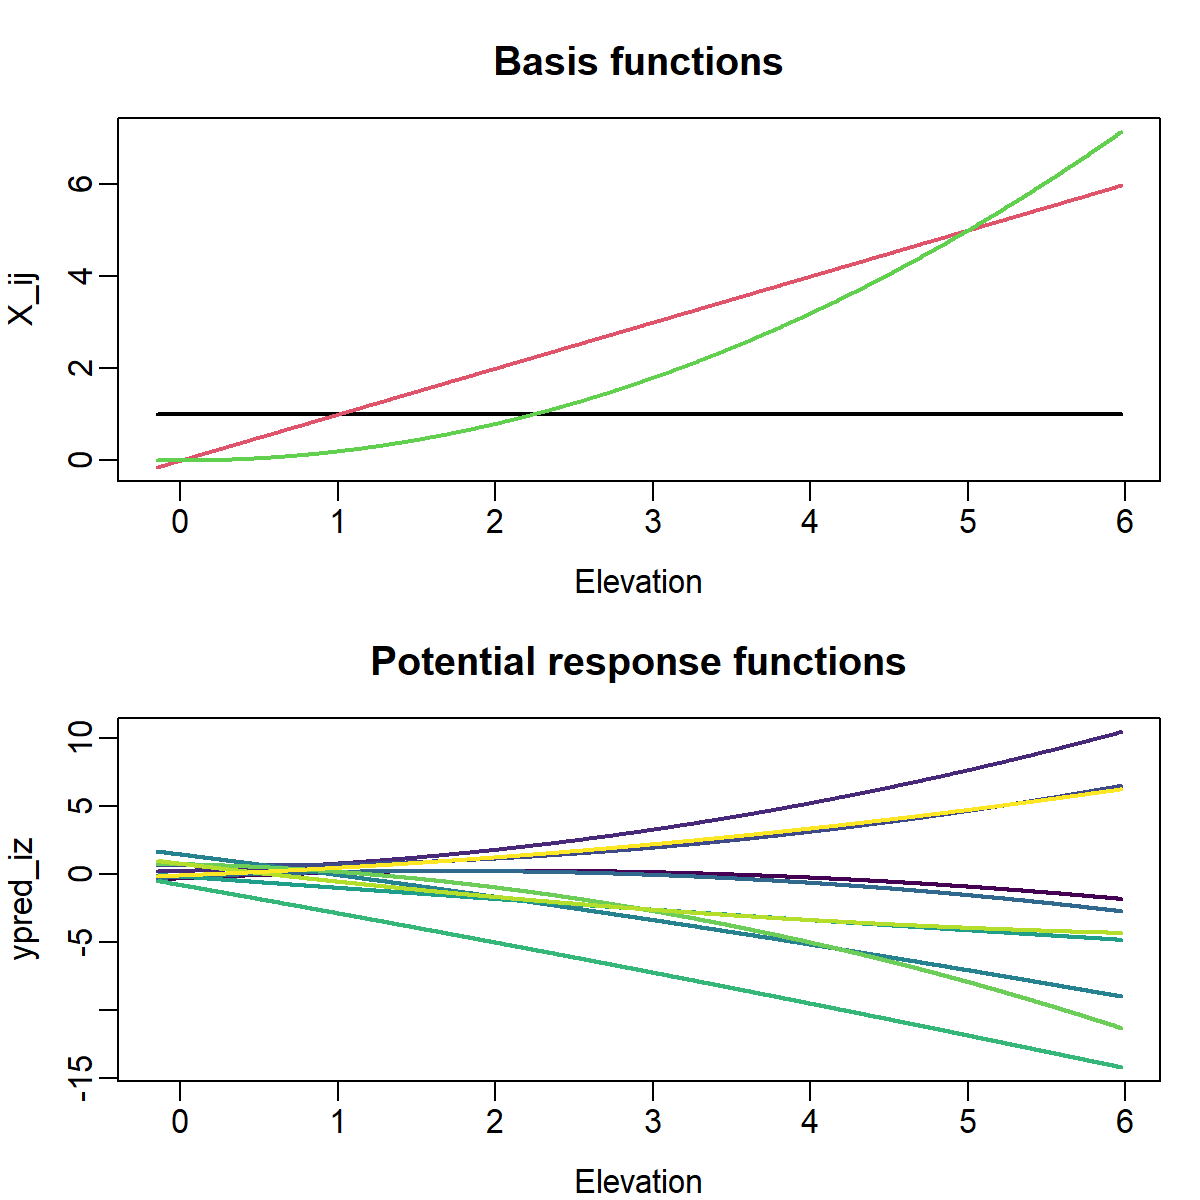
\includegraphics[width=4in]{Chap_5/Basis-polynomial.png}
    \label{fig:Chap5_Basis_polynomial}
\end{figure}

However, higher-order polynomials tend to have extreme slopes and perform poorly when extrapolating outside the observed values for a given covariate.  We therefore next introduce \myindex{splines}.  We will typically use the \colorbox{backcolour}{splines2} package \cite{wang_shape-restricted_2021}, which can construct a conventional B-spline as well as a wide range of alternatives having useful and specialized characteristics.  Constructing a spline involves at least two choices:
\begin{itemize}
    \item \textit{Order}:  splines are designed to vary smoothly, such that the linear predictor \( \mathbf{\mu = X \beta} \) is also a smooth function.  Technically, this involves specifying the spline order, where all derivatives of each basis up to this order are continuous.  By default, software involving splines often uses a 3rd-order (cubic) spline by default, meaning that the 1st and 2nd derivatives vary smoothly, such that the human eye typically can't identify any discontinuity in the resulting response function;
    
    \item \textit{Knots}:  many types of spline also result in a change in some derivative at specific values of a given covariate.  These changes occur at specified locations (often called \myindex{knots}) where a discontinuity occurs in the specified derivative. 
\end{itemize}
The total degrees of freedom for many basic types of splines is the Order plus the number of knots, such that a 3rd-order spline with 7 knots would then have 10 degrees of freedom.  Said another way, using a 3rd-order basis-spline with seven knots for basis expansion would transform a variable that provides one degree of freedom when fitted in a GLM into 10 separate variables that collectively provide 10 degrees of freedom when fitted in a GLM (Fig. \ref{fig:Chap5_Basis_bs}).  If we define the basis expansion as \(\mathbf{X}^*=b(\mathbf{X})\), we then calculate the linear predictor for a generalized linear model as \( g(\mu_i) = \mathbf{x}_i^* \mathbf{\beta} \).  

\begin{figure}[!ht]
    \caption[Basis functions using cubic splines]{Illustation of the basis functions resulting from a single intercept and covariate (top panel) that is transformed using a 3rd-order basis-spline with seven knots (i.e., 10 degrees of freedom) for basis expansion, and 10 random simulations of the density function that could arise from using this basis (bottom panel).}
    \centering
    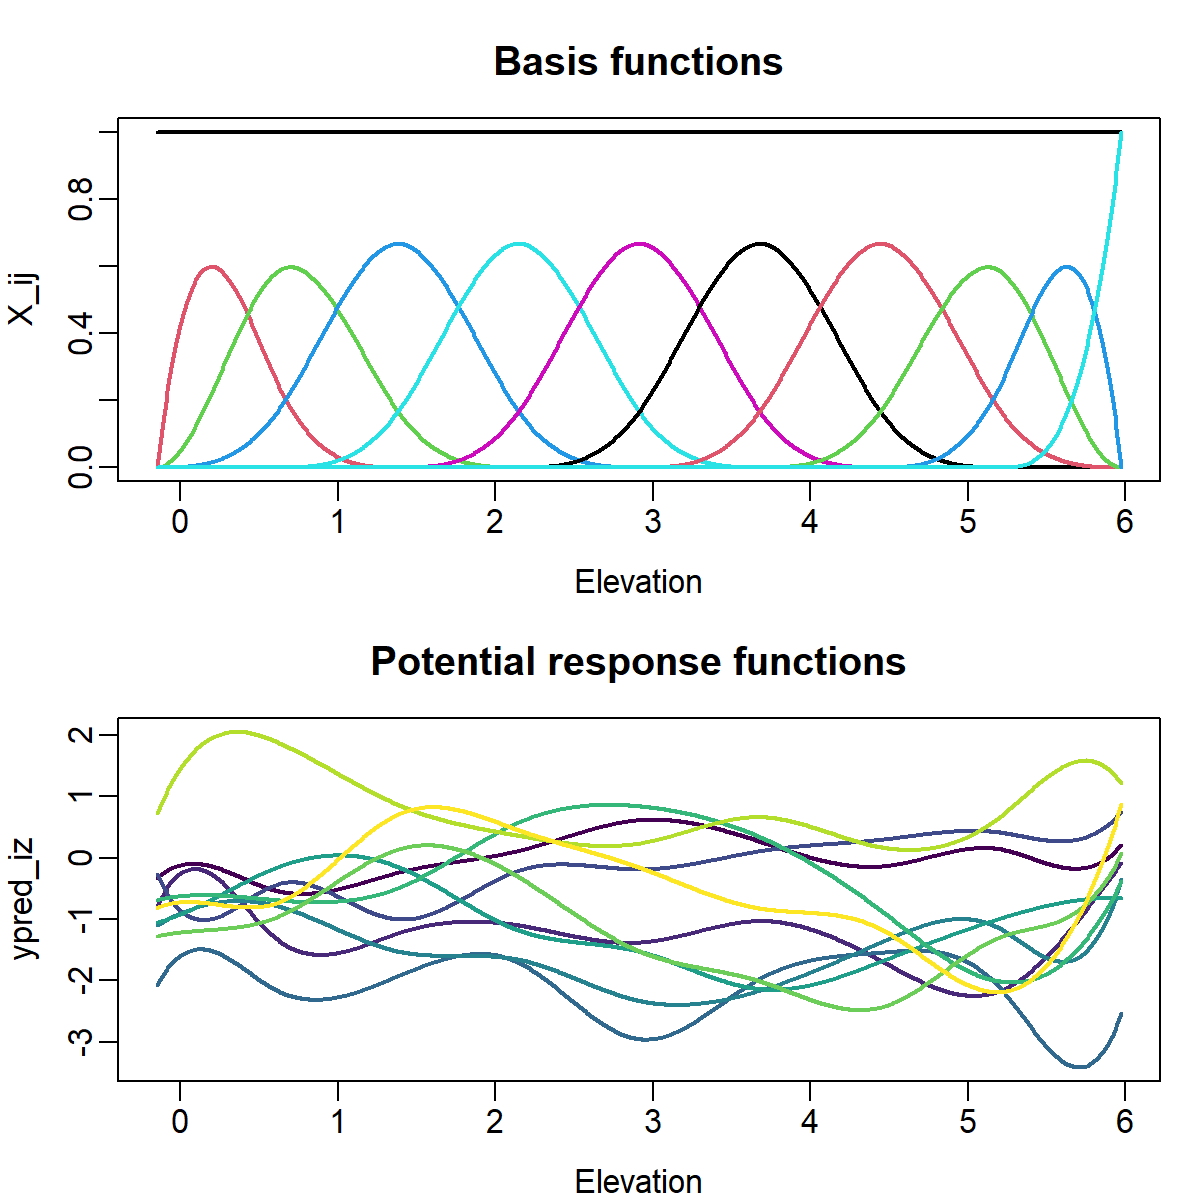
\includegraphics[width=4in]{Chap_5/Basis-bs.png}
    \label{fig:Chap5_Basis_bs}
\end{figure}

To illustrate, we envision that an ecologist might seek to describe the distribution or density of an alpine flower in Mainland China.  This analyst might obtain the elevation throughout mainland China but also want additional flexibility to estimate whether highest densities occur at intermediate elevations.  They might therefore apply spline basis expansion to calculate an expanded set of covariates.  Illustrating this using an intercept and a 3rd-order basis spline with four degrees of freedom (i.e., one internal knot), we see that the first basis function corresponds to lowland areas in eastern and northern China, while the third basis function corresponds largely to the Tibetan plateau (Fig. \ref{fig:Chap5_Basis_maps}).  These five covariates could then be used to provide more flexibility when describing the plant distribution in this hypothetical example.  

\begin{figure}[!ht]
    \caption[Mapped basis functions using cubic splines for elevation]{Illustation of the elevation in Mainland China (top-left panel, in meters above sea level), the intercept, and four basis functions resulting from a basis-spline with four degrees of freedom.}
    \centering
    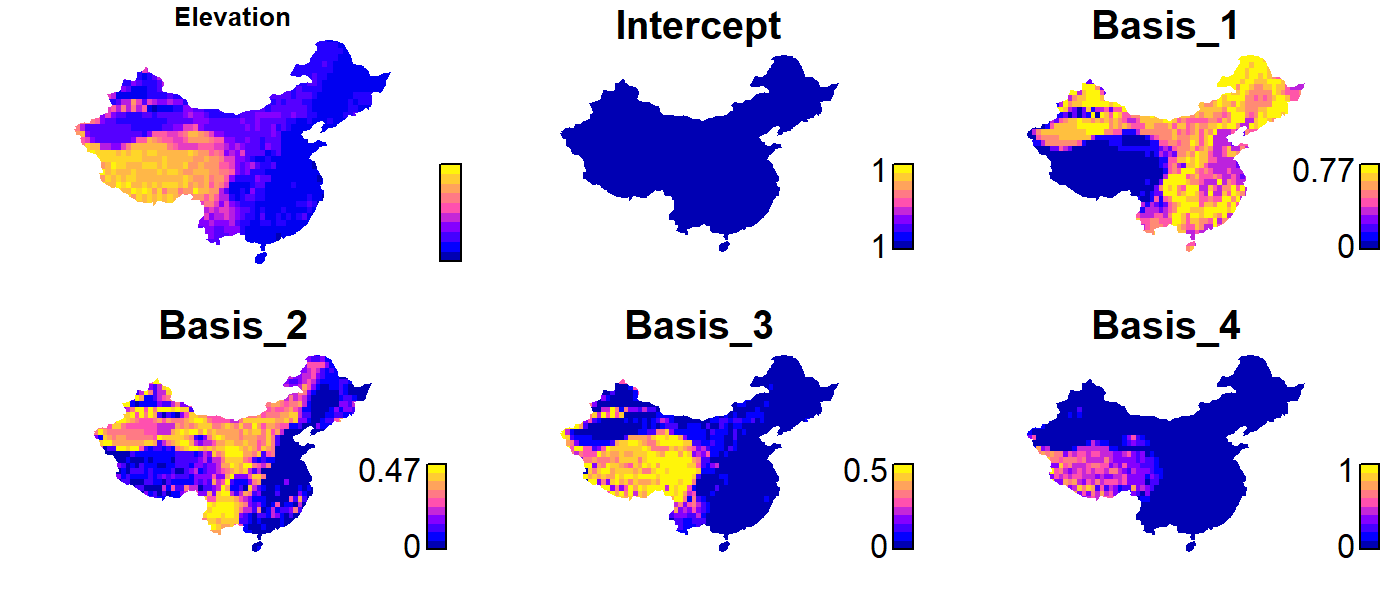
\includegraphics[width=5.5in]{Chap_5/Basis-Map.png}
    \label{fig:Chap5_Basis_maps}
\end{figure}

\section{Tensor Splines and Generalized Additive Models} \label{sec:Chap5_tensor_spliens}

Importantly, splines can be easily defined over multiple dimensions.  For example, vegetation communities depend on the interaction of temperature and precipitation \cite{ricklefs_economy_2008}, such that an analyst might want a spline for the interaction of these two variables.  This then requires a two-dimensional (2D) spline.  A 2D \myindex{tensor spline} can easily be created as:

\begin{equation} \label{eq:Chap5_tensor_spline}
\begin{split}
    \mathbf{z}_i^* \mathbf{\beta} & = \sum_{j=1}^{n_x} \sum_{k=1}^{n_y} \beta_{j,k} \mathrm{x}_{i,j}^* \mathrm{y}_{i,k}^* \\ & = ( \mathrm{x}_{i}^* \otimes \mathrm{y}_{i}^* ) \mathbf{\beta} 
\end{split}
\end{equation}
where \(\otimes\) represents a Kronecker product.  If matrix \(\mathbf{M}_1\) has dimension \( m \times n \) and matrix \(\mathbf{M}_2\) has dimension \( p \times q \), then  \( \mathbf{M}_1\ \otimes\ \mathbf{M}_2\) has dimension \( mp \times nq \).  Restating Eq. \ref{eq:Chap5_tensor_spline}, a tensor-spline is created as the outer product of each individual dimension, where \( b(X,Y) = b(X) \otimes b(Y) \).  If basis \(b(x)\) has \(n_x\) degrees of freedom, and basis \(b(y)\) has \(n_y\) then tensor spline basis \( b(X,Y) \) has \( n_x n_y \) degrees of freedom.

In particular, ecologists often find that fitting a GLM to data that are associated with spatial information (which we call \textit{spatial data} in the following) results in spatially correlated residuals. In these cases, it is feasible to start by including a spline basis-expansion of two-dimensional location.  This is useful for several reasons, e.g.:

\begin{itemize}
    \item \textit{Using available information}:  given the low cost of global position systems (GPS), most ecologists already record the location for each sample.  It is therefore easy and cheap to augment many models with additional information representing geographic location;

    \item \textit{Improved uncertainty estimates}:  GLMs that have spatially correlated residuals violate the assumption that the log-likelihood can be calculated as the sum of log-likelihoods for each datum (see Section \ref{sec:Chap1_likelihood_GLM}).  This violation generally causes standard errors to be too small, and unimportant variables will be identified as statistically significant more often than they should (sometimes called Type-1 error) \cite{dormann_correlation_2012}; 

    \item \textit{Conditional inference}: GLMs that include a basis-expansion of geographic location can then improve predictions.  For example, when predicting density at a location near a positive residual, it might be useful to predict a similarly positive residual at that nearby location.  This involves conditioning the prediction at a given location upon the statistical residuals of nearby locations.
\end{itemize}
For example, expanding our previous discussion of predicting distribution for an alpine plant in mainland China, an analyst might construct a tensor-spline using geographical coordinates.  Using a basis spline with four degrees of freedom for each dimension then results in 16 spline basis functions that each represent a different section of a given spatial domain (Fig. \ref{fig:Chap5_Basis_2D}).  Fitting this model then requires estimating 16 additional parameters.  However, using this tensor spline as a covariate allows a GLM to identify whether the hypothetical plant is associated with broad geographic areas beyond what is explained using elevation.  

\begin{figure}[!ht]
    \caption[Tensor product of cubic spline basis expansion for Latitude-Longitude]{Illustation of the basis functions resulting from Latitude (left column), Longitude (top row), or the two-dimensional tensor-spline basis expansion of Latitude and Longitude arising from the outer product of these two individual dimensions.}
    \centering
    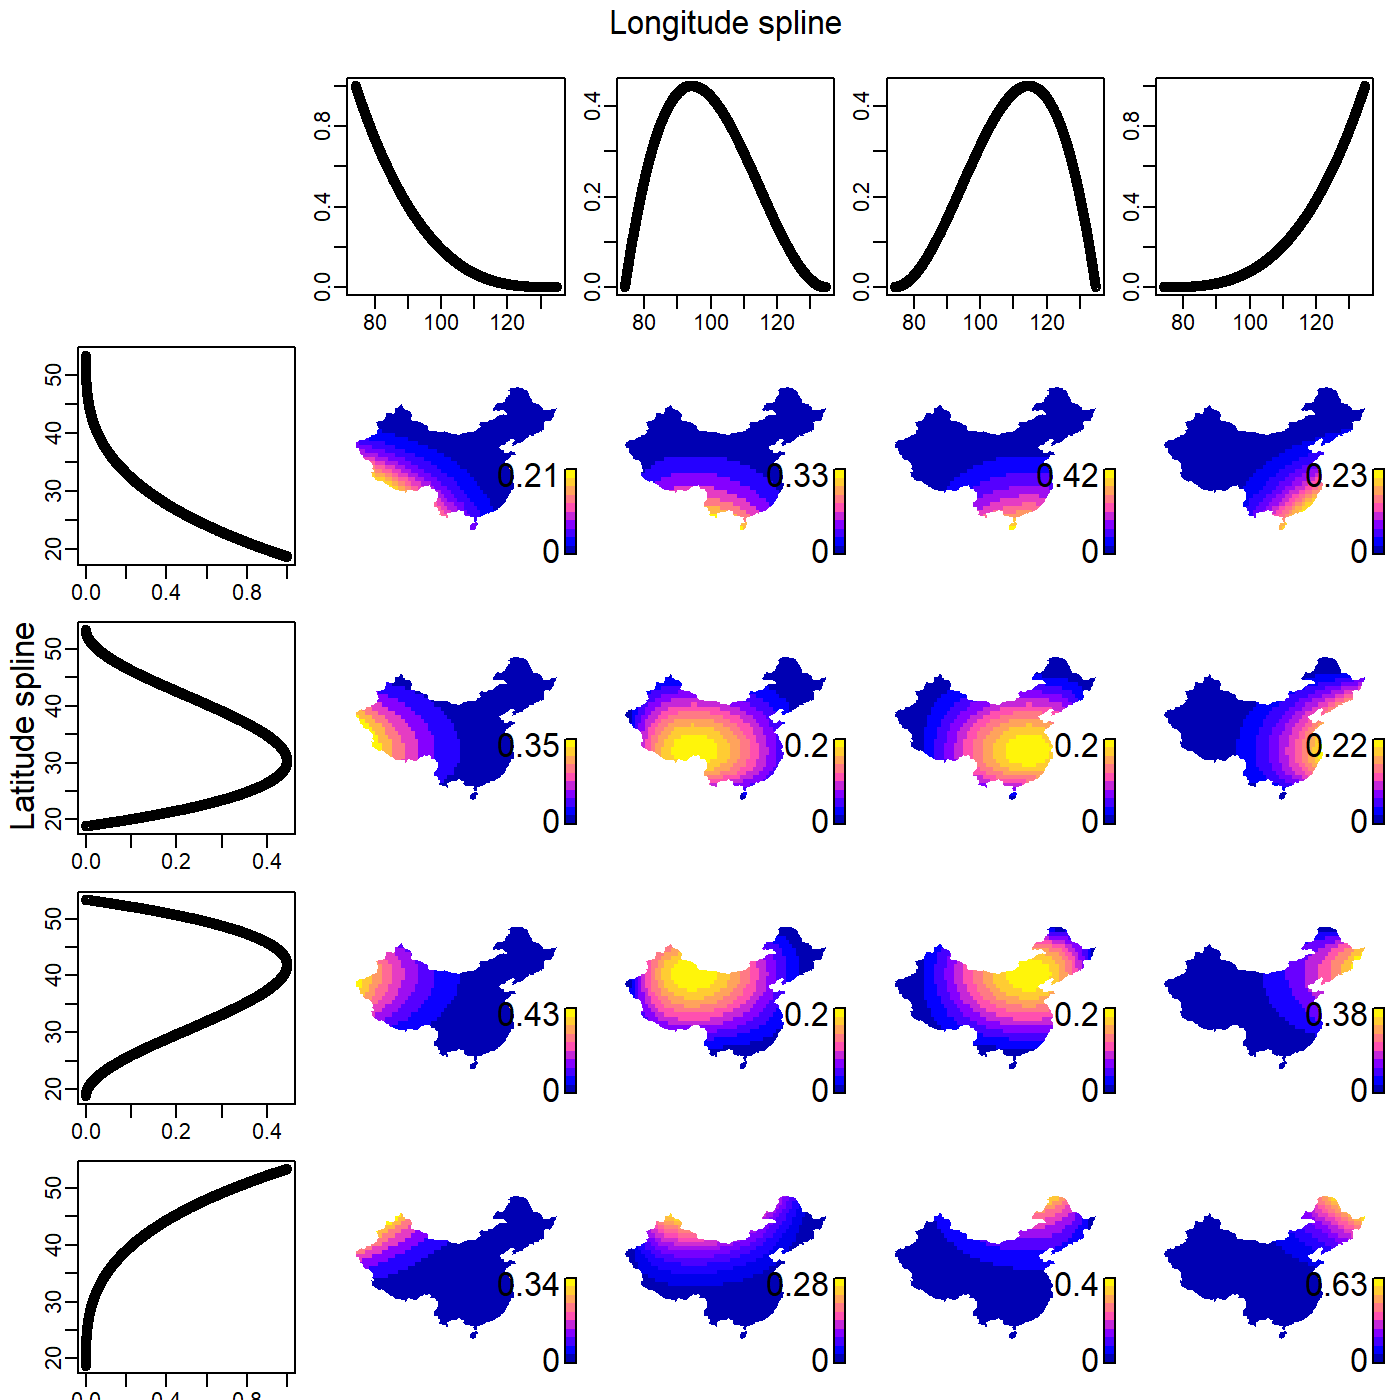
\includegraphics[width=5.5in]{Chap_5/Basis-2D.png}
    \label{fig:Chap5_Basis_2D}
\end{figure}

Next, imagine that we use this 2D basis spline but also choose to shrink the coefficients \(\beta\) towards zero by specifying them as a random effect:

\begin{equation}
\begin{gathered} \label{eq:Chap5_variance}
    g(\mu_i) = \mathbf{X\alpha} + \mathbf{Z\beta} \\
    \beta_k \sim \mathrm{Normal}(0,\sigma^2)
\end{gathered}
\end{equation}
where \( \mathbf{Z} = b(\mathbf{x}, \mathbf{y}) \) is the 2D tensor-spline basis expansion of spatial coordinates and \(\mathbf{X}\) is additional covariates with estimated slopes \(\mathbf{\alpha}\).  To illustrate the consequences of this specification, we note that specifying:

\begin{equation}
\begin{gathered}
    \mathbf{Y} = \mathbf{LX} \\
    \mathbf{X} \sim \mathrm{MVN}(\mathbf{0},\mathbf{\Sigma}) 
\end{gathered}
\end{equation}
is equivalent to specifying:

\begin{equation}
    \mathbf{Y} \sim \mathrm{MVN}(\mathbf{0},\mathbf{L \Sigma} \mathbf{L}^T)     
\end{equation}
so returning to Eq. \ref{eq:Chap5_variance}, we can re-write our GLM as:

\begin{equation}
    g(\mathbf{\mu}) \sim \mathrm{MVN}(\mathbf{X\alpha},\sigma^2 \mathbf{Z} \mathbf{I} \mathbf{Z}^T)
\end{equation}
where the distribution on spline coefficients \(\beta\) implies a covariance \( \sigma^2 \mathbf{Z} \mathbf{I} \mathbf{Z}^T \) for all locations, which depends upon the exact basis functions \(\mathbf{Z}\) being used.

We can therefore specify a generalized linear mixed model (GLMM) using 2D tensor-spline basis functions as covariates, and treating their response coefficients as random effects such that they are shrunk towards zero.  This then allows the smoothness to be estimated as \(\sigma^2\). A sufficiently large value for \(\sigma^2\) results in estimates of \(\beta\) that approach those that would arise from estimating basis functions freely in a GLM (analogous to what we saw in Fig. \ref{fig:Chap2_shrinkage}).  Extending our discussion from Section \ref{sec:Chap2_GLMM}, estimating spline coefficients as random effects is conceptually similar to specifying a GAM, where the log-determinant of the Hessian replaces the penalty term that is using in GAM to restrict the wiggliness of the resulting response function.  

Given this link between GLMMs with spline basis functions and GAMs, ecologists often use widely available software for GAMs to implement spatial models. By default, package \colorbox{backcolour}{mgcv::gam} includes 3rd order splines with many degrees of freedom (e.g., $>$1000 per dimension), and then avoids overparameterization by shrinking coefficients towards zero.  This approach is sometimes called a \myindex{smoothing spline} (or specifically a \textit{thin-plate regression spline}), and the actual placement of knots has little influence on results as the GAM penalty increases \cite{wood_thin_2003}.  

To demonstrate, we download data from the Breeding Bird Survey \cite{sauer_north_1997} using the 2020 release \cite{pardieck_north_2019}\footnote{Data are publicly available, and we downloaded data from \url{https://www.sciencebase.gov/catalog/item/5ea04e9a82cefae35a129d65} on June 14, 2022.}.  This survey started in 1966 and has expanded to include thousands of fixed survey sites across the US and Canada, where these sites are visited annually during peak seasons of May-June.  Each site includes 50 stops located 0.5 miles apart, for a total length of 24.5 miles per survey site.  At each stop within a site, observers spend 3 minutes counting all birds within 0.25 miles of that stop .  We specifically download data for bald eagles \textit{Haliaeetus leucocephalus} in 2018, and restrict data to Alaska, British Columbia and the Yukon (where densities are generally high).  We also combine all stops within a site to calculate the total density at that site.  

We fit these data by specifying a log-linked GAM and using a Poisson distribution.  This GAM is easily fitted using R package \colorbox{backcolour}{mgcv} \cite{wood_fast_2011}:

\lstset{style=Rcode}
\lstinputlisting[language=R, firstline=29, lastline=30, caption=R code to fit a spatial model using R-package \colorbox{backcolour}{mgcv}., captionpos=t]{Chap_5/Spatial_GLMM.R}
where the formula \colorbox{backcolour}{1 + s(X,Y,bs$=$``gp",m$=$1)} specifies a GAM with an intercept and a tensor-product smoothing spline on Latitude and Longitude. We specifically use a first-order penalty and calculate the GAM penalty using a Gaussian process. We specify a Gaussian process for the penalty on the 1st derivative to better match later results, and invite readers to explore the sensitivity to different smoother options available in package \colorbox{backcolour}{mgcv}. This then results in smoothed density estimates, where bald eagles have the highest densities in coastal areas of Alaska and British Columbia (Fig. \ref{fig:Chap5_GAM}).  This GAM can be easily extended to include spatio-temporal variation (i.e., spatial variation that changes over time) by including additional terms in the function \colorbox{backcolour}{s(.)} used to construct the smoothing spline.  

\begin{figure}[!ht]
    \caption[GAM estimates of bald eagle densities]{Estimated summertime log-density of bald eagles in Alaska, British Columbia, and the Yukon Territory, estimated using a GAM fitted to Breeding Bird survey counts (see colorbar for scale of log-densities in units numbers per survey station), showing either the full results (ranging widely from \(e^4=55\) to \(e^{-40} \leq 10^{-15}\) birds per station) as well as results that trim densities less than 0.1\% of the maximum estimated density (to better show contrast in results in areas with non-zero densities).}
    \centering
    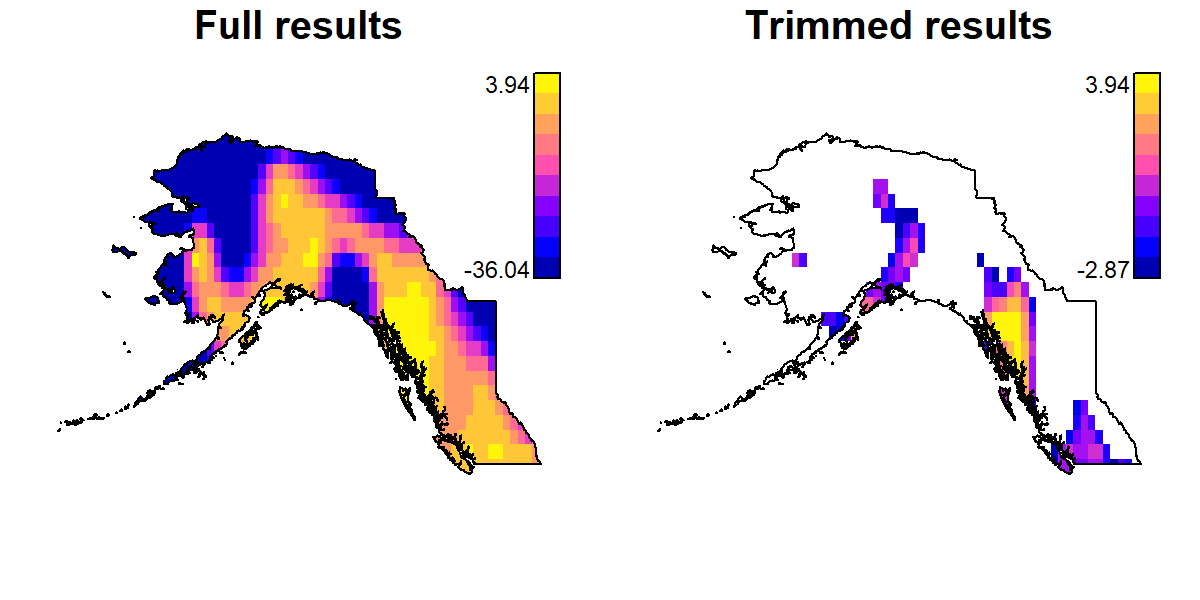
\includegraphics[width=4in]{Chap_5/Mapped_GAM.png}
    \label{fig:Chap5_GAM}
\end{figure}

\section{Separable Correlation and Sparsity} \label{sec:Chap5_separable_correlation}

As an alternative to specifying 2D tensor-product basis functions as covariates to estimate residual spatial variation, we next extend autoregressive models to two dimensions.  Specifically, we seek to define the probability distribution for a random effect \(\omega_{x,y}\), where coordinates \((x,y)\) are defined on an evenly spaced grid.

As we saw in Section \ref{sec:Chap3_joint_Gompertz}, we can fit an autoregressive model by specifying either a series of conditional distributions, or by constructing the precision of their joint distribution.  One way to generalize autoregression to two dimensions on an evenly spaced grid involves combining these:

\begin{equation}
\begin{gathered}
    \mathbf{\omega}_{y} \sim 
    \begin{cases}
        \mathrm{MVN}\left(\mathbf{0},\frac{\sigma^2}{1-\rho^2} \mathbf{R}\right) & \text{if } y=1 \\ 
        \mathrm{MVN}\left(\rho \mathbf{\omega}_{y-1},\sigma^2 \mathbf{R}\right) & \text{if } y>1 
    \end{cases} \\
\end{gathered}
\end{equation}
where this defines the joint distribution for each row of \(\omega_{y+1}\) conditional upon its value in the row before \(\omega_{y}\). We can write a custom function \colorbox{backblue}{conditional\_distribution} that evaluates this probability density in TMB (Code \ref{code:Chap5-conditional-distribution}), where we first construct the precision matrix \colorbox{backblue}{Q\_yy} for each row of the matrix \colorbox{backblue}{epsilon\_xy} of random, and loop through rows applying a custom function \colorbox{backblue}{dmvnorm} to evaluate the conditional probability.  

\lstset{style=TMBcode}
\lstinputlisting[language=c++, label=code:Chap5-conditional-distribution, caption=TMB code defining a custom function to assemble a precision matrix for a one-dimensional autoregressive process and looping that across a second dimension., captionpos=t]{Chap_5/conditional_distribution.hpp}

Alternatively, we can write a custom function \colorbox{backblue}{joint\_distribution} (Code \ref{code:Chap5-joint-distribution}) that evaluates the same probability density by constructing the Kronecker product of the 2-dimensional autoregressive process:

\begin{equation} \label{eq:Chap5_joint}
    \mathrm{vec}(\omega) \sim \mathrm{MVN}(\mathbf{0},\sigma^2 \mathbf{R}_1 \otimes \mathbf{R}_2)
\end{equation}
This function constructs the two precision matrices \colorbox{backblue}{Q\_xx} and \colorbox{backblue}{Q\_yy} and then uses the internal function \colorbox{backblue}{kronecker} to construct the precision \colorbox{backblue}{Q\_zz}.  Any correlation or precision matrix that can be constructed as the Kronecker product of two smaller matrices is called a \myindex{separable} process, and constructing the precision in this way is the key to constructing computationally efficient distributions for high-dimensional processes. Again extending what we saw in Section \ref{sec:Chap3_joint_Gompertz}, we can equivalently write this as:

\begin{equation}
    \mathrm{vec}(\omega) \sim \mathrm{MVN}(\mathbf{0},\sigma^{-2} \mathbf{Q}_1^{-1} \otimes \mathbf{Q}_2^{-1})
\end{equation}
where \(\mathbf{Q}\) is the precision matrix for the autoregressive process in one dimension.  As we saw before, each individual precision matrix can be formed analytically (Eq. \ref{eq:Chap3_joint_precision}) and is sparse (i.e., nonzero only for adjacent cells).  

\lstset{style=TMBcode}
\lstinputlisting[language=c++, label=code:Chap5-joint-distribution, caption=TMB code defining a custom function to assemble a precision matrix for a two-dimensional autoregressive process., captionpos=t]{Chap_5/joint_distribution.hpp}

Combining two precision matrices in a separable model then has several useful properties:

\begin{itemize}
    \item \textit{Sparsity}:  if we define the proportion of nonzero elements in matrix \(\mathbf{M}_1\) as its sparsity \(p_1\), and the proportion in correlation \(\mathbf{M}_2\) as \(p_2\), then the sparsity of \( \mathbf{M}_1 \otimes \mathbf{M}_2 \) is \(p_1 p_2\). Said another way, a separable precision matrix is more sparse than each dimension individually.  For example, in the case of this 2D equally spaced grid, the sparsity pattern of the inner Hessian (Fig. \ref{fig:Chap5_Hessian}) matches the sparsity of the precision matrices \( \mathbf{Q}_1^{-1} \otimes \mathbf{Q}_2^{-1} \);

    \item \textit{Modularity}:  if we learn how to construct the precision or covariance matrix arising from a few elementary processes (e.g., an equally spaced grid in Eq. \ref{eq:Chap3_joint_precision}, or a structural equation model in Eq. \ref{eq:Chap4_SEM_covariance}), we can then mix-and-match which matrix is the best for describing covariance over space vs. over time vs. among variables.  We can then construct the joint covariance from the Kroenecker product of these individual matrices.
\end{itemize}

\begin{figure}[!ht] 
    \caption[Sparsity pattern for 2D autoregressive spatial GLMM]{Sparsity pattern arising from a 2D equally spaced grid with 21 rows and 52 columns (1092 elements total), showing the banded pattern that is typical for a separable correlation.}
    \centering
    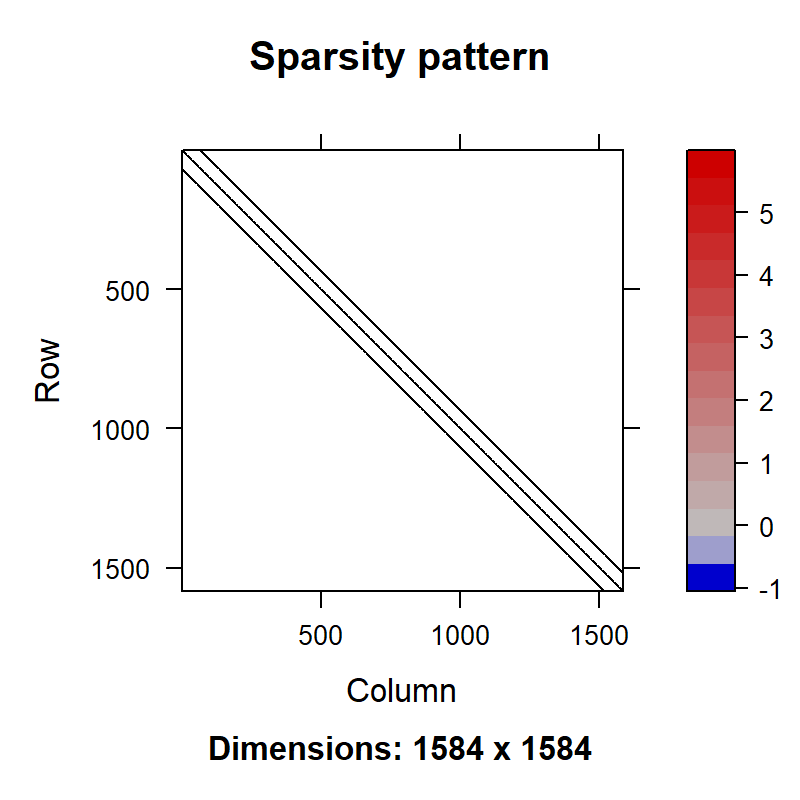
\includegraphics[width=4in]{Chap_5/Hessian.png}
    \label{fig:Chap5_Hessian}
\end{figure}

\begin{table}
  \caption[TMB functions in the \colorbox{backblue}{density} namespace to specify spatial models]{A brief summary of some functions available in namespace \colorbox{backblue}{density}, which can be used to simplify code when implementing a separable spatial or spatio-temporal model using TMB.}
\begin{center}
\begin{tabularx}{\linewidth}{ | X m{3in} | } 
  \hline
  Function in \colorbox{backblue}{density} namespace & What it does \\ 
  \hline

  \colorbox{backblue}{GMRF\_t\textlangle Type\textrangle  gmrf} & Constructs an object named \colorbox{backblue}{gmrf} of class \colorbox{backblue}{GMRF\_t}, where users can later call \colorbox{backblue}{jnll += gmrf(user\_vector)} to evaluate the negative log-likelihood of a user-supplied vector \colorbox{backblue}{user\_vector} given a distribution defined by \colorbox{backblue}{gmrf} \\ & \\ 

  \colorbox{backblue}{gmrf = GMRF(precision)} & Given a specified precision matrix \colorbox{backblue}{precision}, define a \colorbox{backblue}{GMRF\_t} object with covariance defined as the inverse of \colorbox{backblue}{precision} \\ & \\ 
  
  \colorbox{backblue}{gmrf = AR1(rho)} & Defines a \colorbox{backblue}{GMRF\_t} object such that it evaluates the probability distribution arising from a regularly spaced, first-order autoregressive process with autocorrelation \colorbox{backblue}{rho} and unit variance \\ & \\ 
  
  \colorbox{backblue}{gmrf = SCALE(gmrf1, sd)} & Given a specified \colorbox{backblue}{GMRF\_t} object, rescales it to have standard deviation \colorbox{backblue}{sd} \\ & \\ 

  \colorbox{backblue}{gmrf = SEPARABLE(gmrf1, gmrf2)} & Given two \colorbox{backblue}{GMRF\_t} objects, \colorbox{backblue}{gmrf1} and \colorbox{backblue}{gmrf2}, construct a new \colorbox{backblue}{GMRF\_t} object with covariance that arises as the Kronecker product of the covariance for \colorbox{backblue}{gmrf1} and \colorbox{backblue}{gmrf2} \\ 
  
  \hline
\end{tabularx}
  \label{tab:Chap5_density_package}
\end{center}
\end{table}

Alternatively, TMB includes a namespace \colorbox{backblue}{density} that includes functions that can automate many of these steps when constructing a separable spatial model (see Table \ref{tab:Chap5_density_package} for a list).  We next show how to fit the two-dimenstional spatial model using these functions.  Specifically:
\begin{itemize}
    \item \colorbox{backblue}{AR1(rho)} constructs the precision matrix for an evenly spaced autoregressive process with conditional standard deviation of \(1\);

    \item \colorbox{backblue}{SEPARABLE(AR1(rho),AR1(rho))} constructs the separable precision arising from two AR1 processes;

    \item \colorbox{backblue}{SCALE( SEPARABLE(AR1(rho),AR1(rho)), scale )} takes a separable precision with a standard deviation of 1 and rescales it to have a standard deviation of \colorbox{backblue}{scale};

    \item \colorbox{backblue}{SCALE( SEPARABLE(AR1(rho), AR1(rho)), scale )( epsilon\_xy )} takes this rescaled and separable precision, and calculates the negative log-likelihood of \colorbox{backblue}{epsilon\_xy} arising from that distribution.
\end{itemize}
In summary, a few statements in TMB then implements the entire calculation for the separable covariance function (Code \ref{code:Chap5-TMB-precision-constructors}), while internally tracking the inverse covariance (``precision") matrix for efficient computation.  

\lstset{style=TMBcode}
\lstinputlisting[language=c++, label=code:Chap5-TMB-precision-constructors, firstline=33, lastline=52, caption=TMB code comparing three alternative ways to implement a two-dimensional autoregressive process for a spatial generalized linear mixed model., captionpos=t]{Chap_5/autoregressive_grid.cpp}

We again fit these models to data for bald eagles in Alaska, British Columbia, and Yukon in 2019.  Comparing these three implementations of a 2D autoregressive for these data shows that they give similar parameter estimates (Table \ref{tab:Chap5_comparing_parameters}), where differences arise from different treatments of boundary effects.  However, the implementation that constructs the joint precision matrix takes much longer to run, because it does not efficiently use information about the sparcity of the inner Hessian matrix when calculating the log-determinant as used in the Laplace approximation (Eq. \ref{eq:Chap2_laplace}).  Similarly, these three models all estimate density maps that are generally similar (Fig. \ref{fig:Chap5_mapped_densities}).  We note that the GAM results included density estimates of less than one bird per quadrillion stations, which intuitively seems like an extreme value to predict.  By contrast, the various two-dimensional autoregressive models predict low densities of approximately one bird per 100 stations, which seems like a more reasonable estimate for the lower range of densities.   

\begin{table} 
    \caption[Comparing three specifications for two-dimensional spatial GLMM]{Comparing the estimated intercept, natural-log of spatial variance, the logit-transformed spatial autocorrelation, and the runtime in seconds for three alternative implementations of a log-linked Poisson-GLM fitted using TMB.  These three specify the joint distribution for each row of the spatial process conditional upon the previous row, construct the joint precision as the Kronecker product of one-dimensional autoregressive terms, or using the built-in \colorbox{backblue}{density} package.}
    \catcode`"=9
  \centering
    \csvautotabular[respect all]{Chap_5/Comparison.csv}
    \label{tab:Chap5_comparing_parameters}
\end{table} 

\begin{figure}[!ht]
    \caption[GLMM estimates of bald eagle densities using three alternative methods]{Estimated summertime log-density of bald eagles in Alaska, British Columbia, and the Yukon Territory, estimated using a GLMM fitted to Breeding Bird survey counts using three alternative versions of a 2D autoregressive process that estimates density across an entire grid but only showing those cells that overlap with an intended spatial domain.}
    \centering
    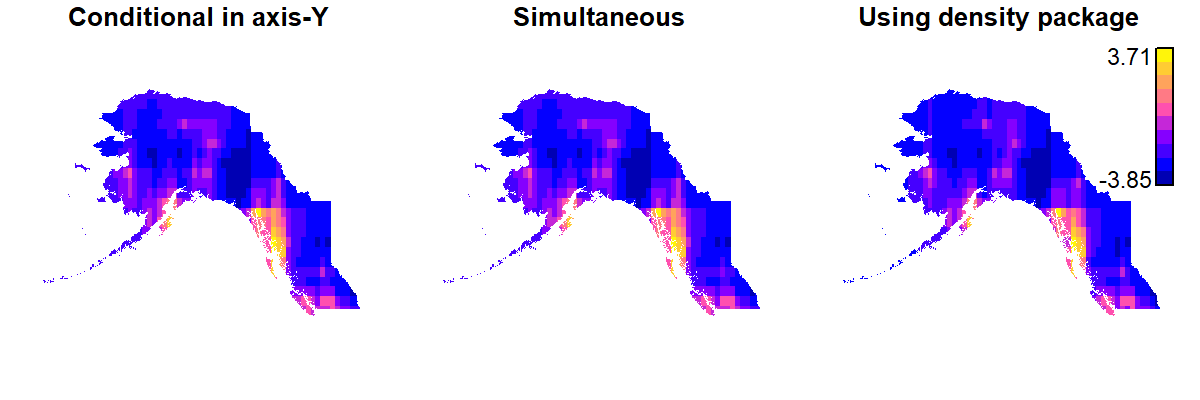
\includegraphics[width=5.5in]{Chap_5/Mapped_densities.png}
    \label{fig:Chap5_mapped_densities}
\end{figure}

We can further visualize the properties of the covariance matrix resulting from a 2D autoregressive process \(\mathbf{\Sigma}_{full} = \sigma^{-2} \mathbf{Q}_1^{-1} \otimes \mathbf{Q}_2^{-1}\) via it's \myindex{eigendecomposition}.  Specifically, any covariance can be decomposed as:

\begin{equation} \label{eq:Chap5_eigen}
    \mathbf{\Sigma} = \mathbf{V \Lambda V}^T
\end{equation}
where the eigendecomposition is defined as \( \mathrm{eigen}: \mathbf{\Sigma} \mapsto ( \mathbf{V, \lambda} ) \), such that eigenvectors \(\mathbf{V}\) are orthogonal to one-another and have length of one, and eigenvalues \(\lambda\) measure the variance associated with each eigenvector (see Section \ref{sec:Appendix_eigendecomposition} for more details).  As a consequence of Eq. \ref{eq:Chap5_variance}, we can rewrite \ref{eq:Chap5_joint} as:

\begin{gather*}
    \mathrm{vec}(\omega) = \mathbf{V \Lambda}^{0.5} \mathrm{vec}(\omega^*) \\
    \mathrm{vec}(\omega^*) \sim \mathrm{MVN}(\mathbf{0},\mathbf{I})
\end{gather*} 
where \( \mathbf{\Sigma}_{full} = \mathbf{V \Lambda}^{0.5} (\mathbf{V \Lambda}^{0.5})^T \).  In a sense, then, \( \mathbf{V \Lambda}^{0.5} \) are the basis functions associated with covariance \( \mathbf{\Sigma}_{full} \).  If we map the first basis functions (Fig. \ref{fig:Chap5_AR_basis_functions}), we see that the largest basis functions capture correlations over broad spatial scales, e.g., where v.2 represents variation from west to east and therefore distinguishes British Columbia and the Yukon Territory from central and western Alaska.  Although these basis functions differ from the tensor-spline basis functions constructed previously (Fig. \ref{fig:Chap5_Basis_2D}), the dominant eigenvectors serve a similar role in representing broad-scale spatial patterns.  Furthermore, estimating this model as a GLMM shrinks coefficients towards zero based on the marginal likelihood, and this shrinkage is conceptually similar to the penalty term that occurs in a GAM.  We therefore see that the GLMM using a 2D autoregressive correlation is similar to a GAM that is specified using the same basis functions.  

\begin{figure}[!ht]
    \caption[Example of basis functions for 2D autoregressive process]{First 16 basis functions for the bald eagle species distribution model, showing \( \mathbf{V \Lambda}^{0.5} \) from the eigendecomposition of the covariance matrix resulting from a separable 2D autoregressive process.}
    \centering
    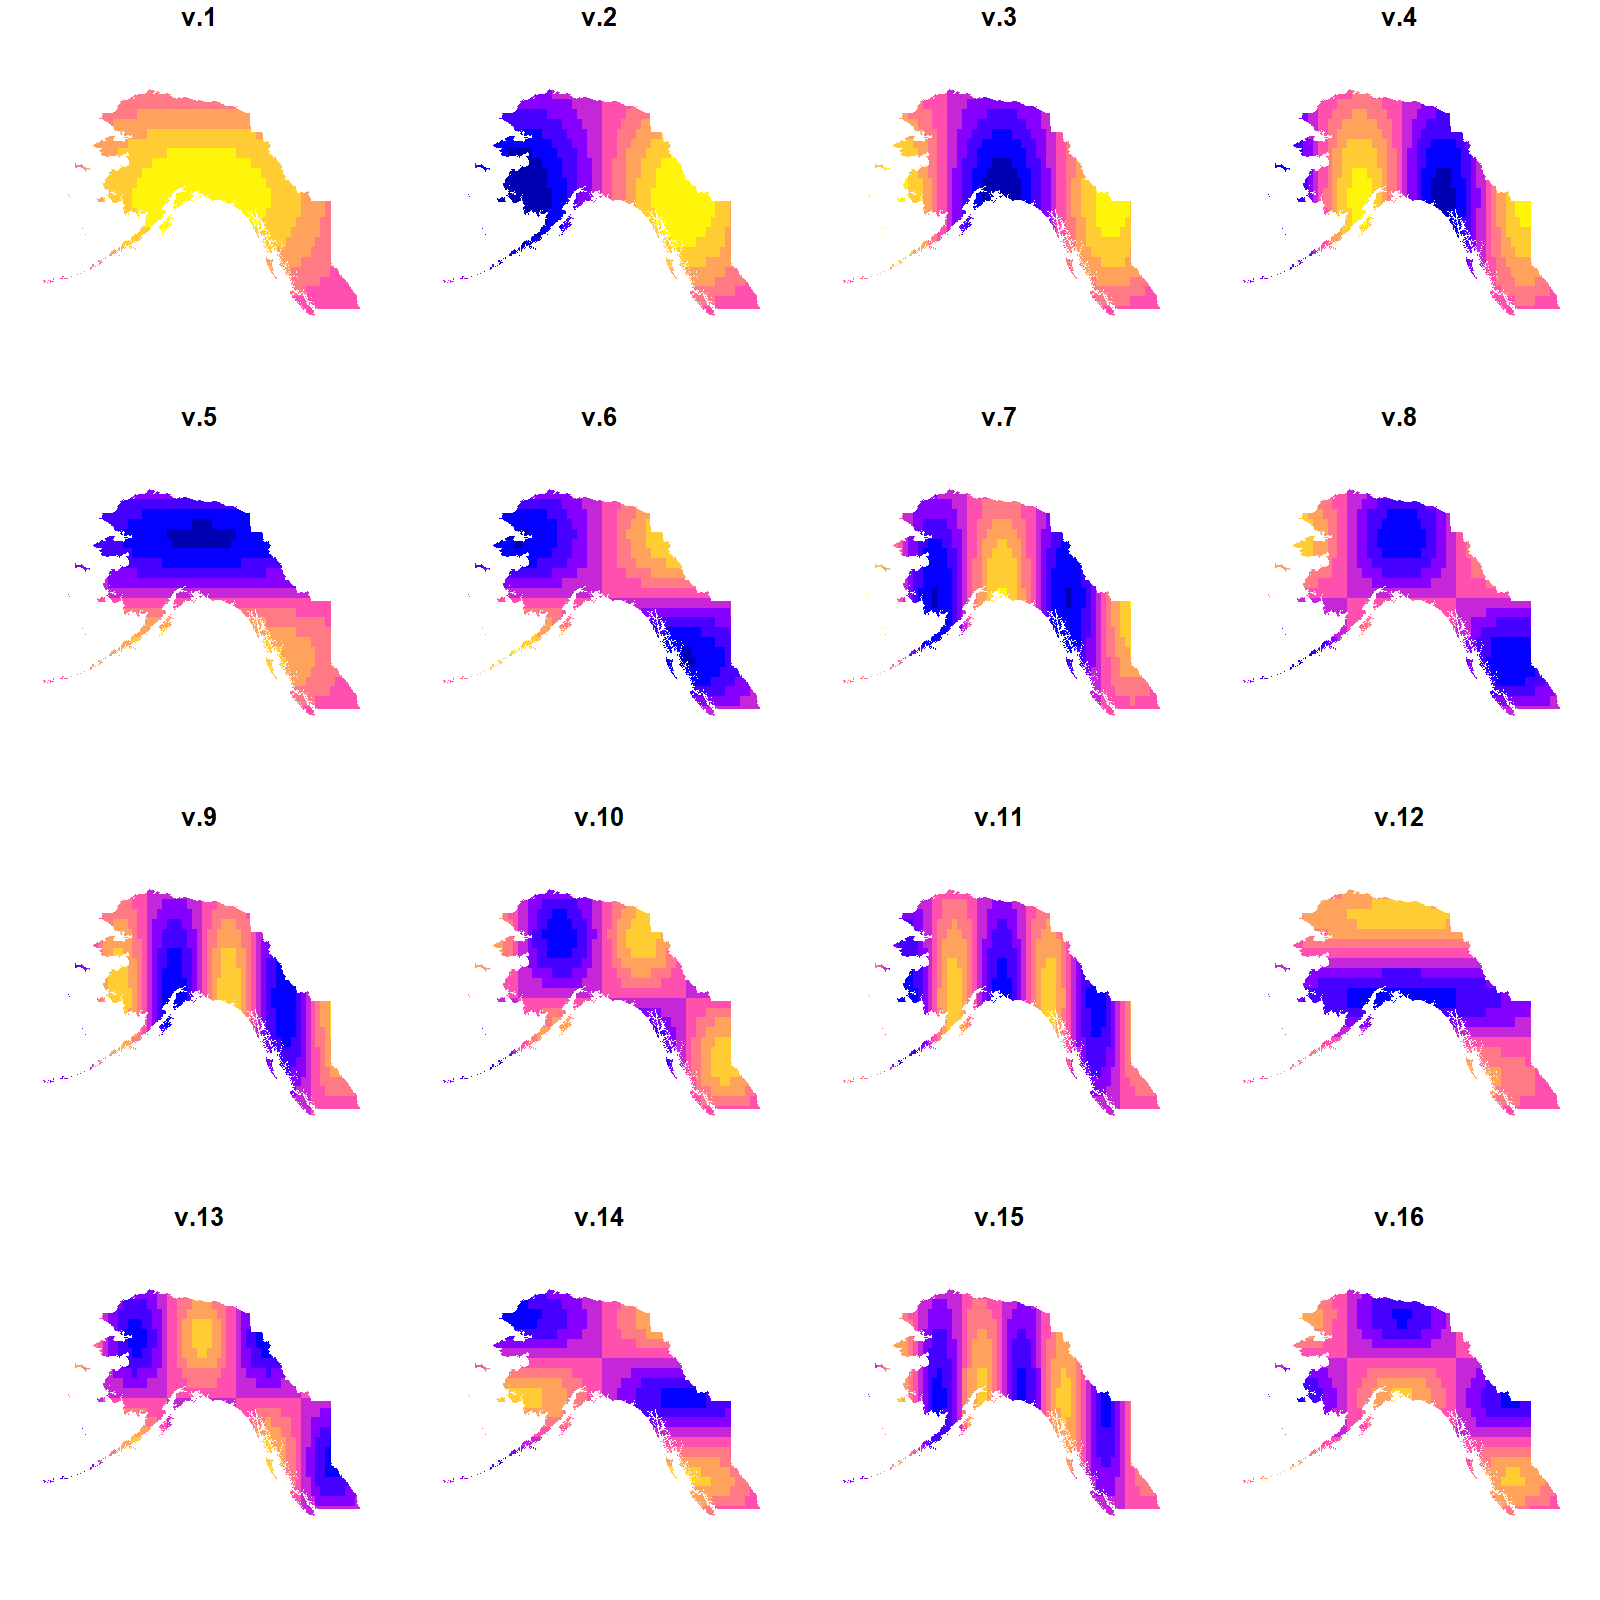
\includegraphics[width=5.5in]{Chap_5/Mapped_AR_basis_functions.png}
    \label{fig:Chap5_AR_basis_functions}
\end{figure}

\section{Models for Irregular Shaped Spatial Domains} \label{sec:Chap5_irregular_spatial_covariance}

Despite the speed and convenience of specifying a 2D autoregressive process using separable functions via package \colorbox{backblue}{density}, this approach  wastes computational resources estimating random effects for grid cells that are outside of the spatial domain (in this case over water), which we then ignore when interpreting the output.  This issue is analogous to defining state-space models over a single temporal dimension, but defined for uneven time intervals, as we discussed previously in Section \ref{sec:Chap3_seasonal}.  It is therefore helpful to define a precision matrix for unevenly spaced locations in two-dimensional space. There are many different approaches to do so \cite{vecchia_estimation_1988}, but we here focus on two methods: the conditional autoregressive model, and the stochastic partial differential equation (SPDE) method. 

\subsection{Conditional Autoregressive Model} \label{sec:Chap5_CAR}

Spatial modelling has typically emphasized \textit{conditional autoregressive} and \textit{simultaneous autoregressive} approaches that can directly construct the precision matrix for a spatially correlated variable \cite{cressie_statistics_1993}.  We previously introduced the simultaneous autoregressive process in Section \ref{sec:Chap3_state_space}, and see Appendix \ref{sec:Appendix_SAR} for a derivation of a SAR for a one-dimensional autoregressive process.  We here introduce the alternative \myindex{conditional autoregressive process} or CAR model.  

\begin{figure}[!ht]
    \caption[Estimates of eagle densities using conditional autoregressive model]{Estimated bald eagle densities, using a GLMM fitted to Breeding Bird survey counts using a conditional autoregressive model that only requires fitting to those grid cells that are within the intended spatial domain.}
    \centering
    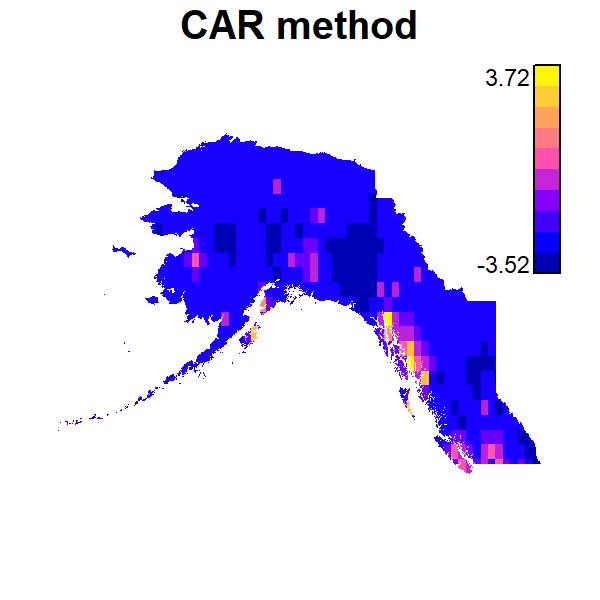
\includegraphics[width=3in]{Chap_5/Mapped_densities--CAR.png}
    \label{fig:Chap5_CAR_densities}
\end{figure}

To define the CAR model, we divide a spatial domain into a set of \( n_g \) polygons (a.k.a. cells) that are non-overlapping and contain the entire domain.  We then  introduce the \myindex{adjacency matrix} \( \mathbf{A} \) with dimension \(n_g\) by \(n_g\).  The adjacency matrix \( \mathbf{A} \) has a value \( a_{i,j} = 1 \) if cell \(i\) is adjacent to cell \(j\) and \( a_{i,j} = 0 \) otherwise.  We here will divide a spatial area into square grid cells, and define adjacency as grid cells that share an edge (not just a vertex).  This implies that a square grid cell is adjacent to at most four other cells;  this is sometimes called \myindex{rook adjacency}, similar to how a rook is allowed to move along rows or columns in the game of chess.  The adjacency matrix is typically sparse and depends entirely on the spatial configuration and shape of modeled cells.  Alternative definitions of adjacency are possible which also result in a sparse adjacency matrix.  For example, \myindex{queen adjacency} defines two polygons as adjacent if they share either an edge or a vertex, such that a square grid cell could be adjacent to at most 8 neighboring cells.  The following methods can be applied to these different definitions of adjacency, although we will use rook-adjacency for simplicity of presentation.

Given evenly sized grid cells and adjacency matrix \( \mathbf{A} \), a CAR model constructs the inverse covariance \( \mathbf{Q} \) as:

\begin{equation} \label{eq:Chap5_CAR}
    \mathbf{Q} = \frac{1}{\sigma^2} (\mathbf{I} - \rho \mathbf{A})
\end{equation}
where this construction is nonzero only on the diagonal or for adjacent cells \cite{ver_hoef_relationship_2018}.  However, this simple construction comes with the drawback that \( \rho \) has a less intuitive interpretation than other methods.  In particular, this equation only results in a valid precision matrix if \( \frac{1}{\lambda_{min}} < \rho < \frac{1}{\lambda_{max}} \), where \( \lambda_{min} \) and \( \lambda_{max} \) are the minimum and maximum eigenvalues of adjacency matrix \( \mathbf{A} \).  We specifically use R-package \colorbox{backcolour}{igraph} \cite{csardi_igraph_2006} to calculate these minimum and maximum eigenvalues efficiently given that \( \mathbf{A} \) is sparse.  

\begin{figure}[!ht]
    \caption[Example of basis functions for CAR model]{First 16 basis functions for the bald eagle species distribution model, showing \( \mathbf{V \Lambda}^{0.5} \) from the eigendecomposition of the covariance matrix resulting from a CAR model.}
    \centering
    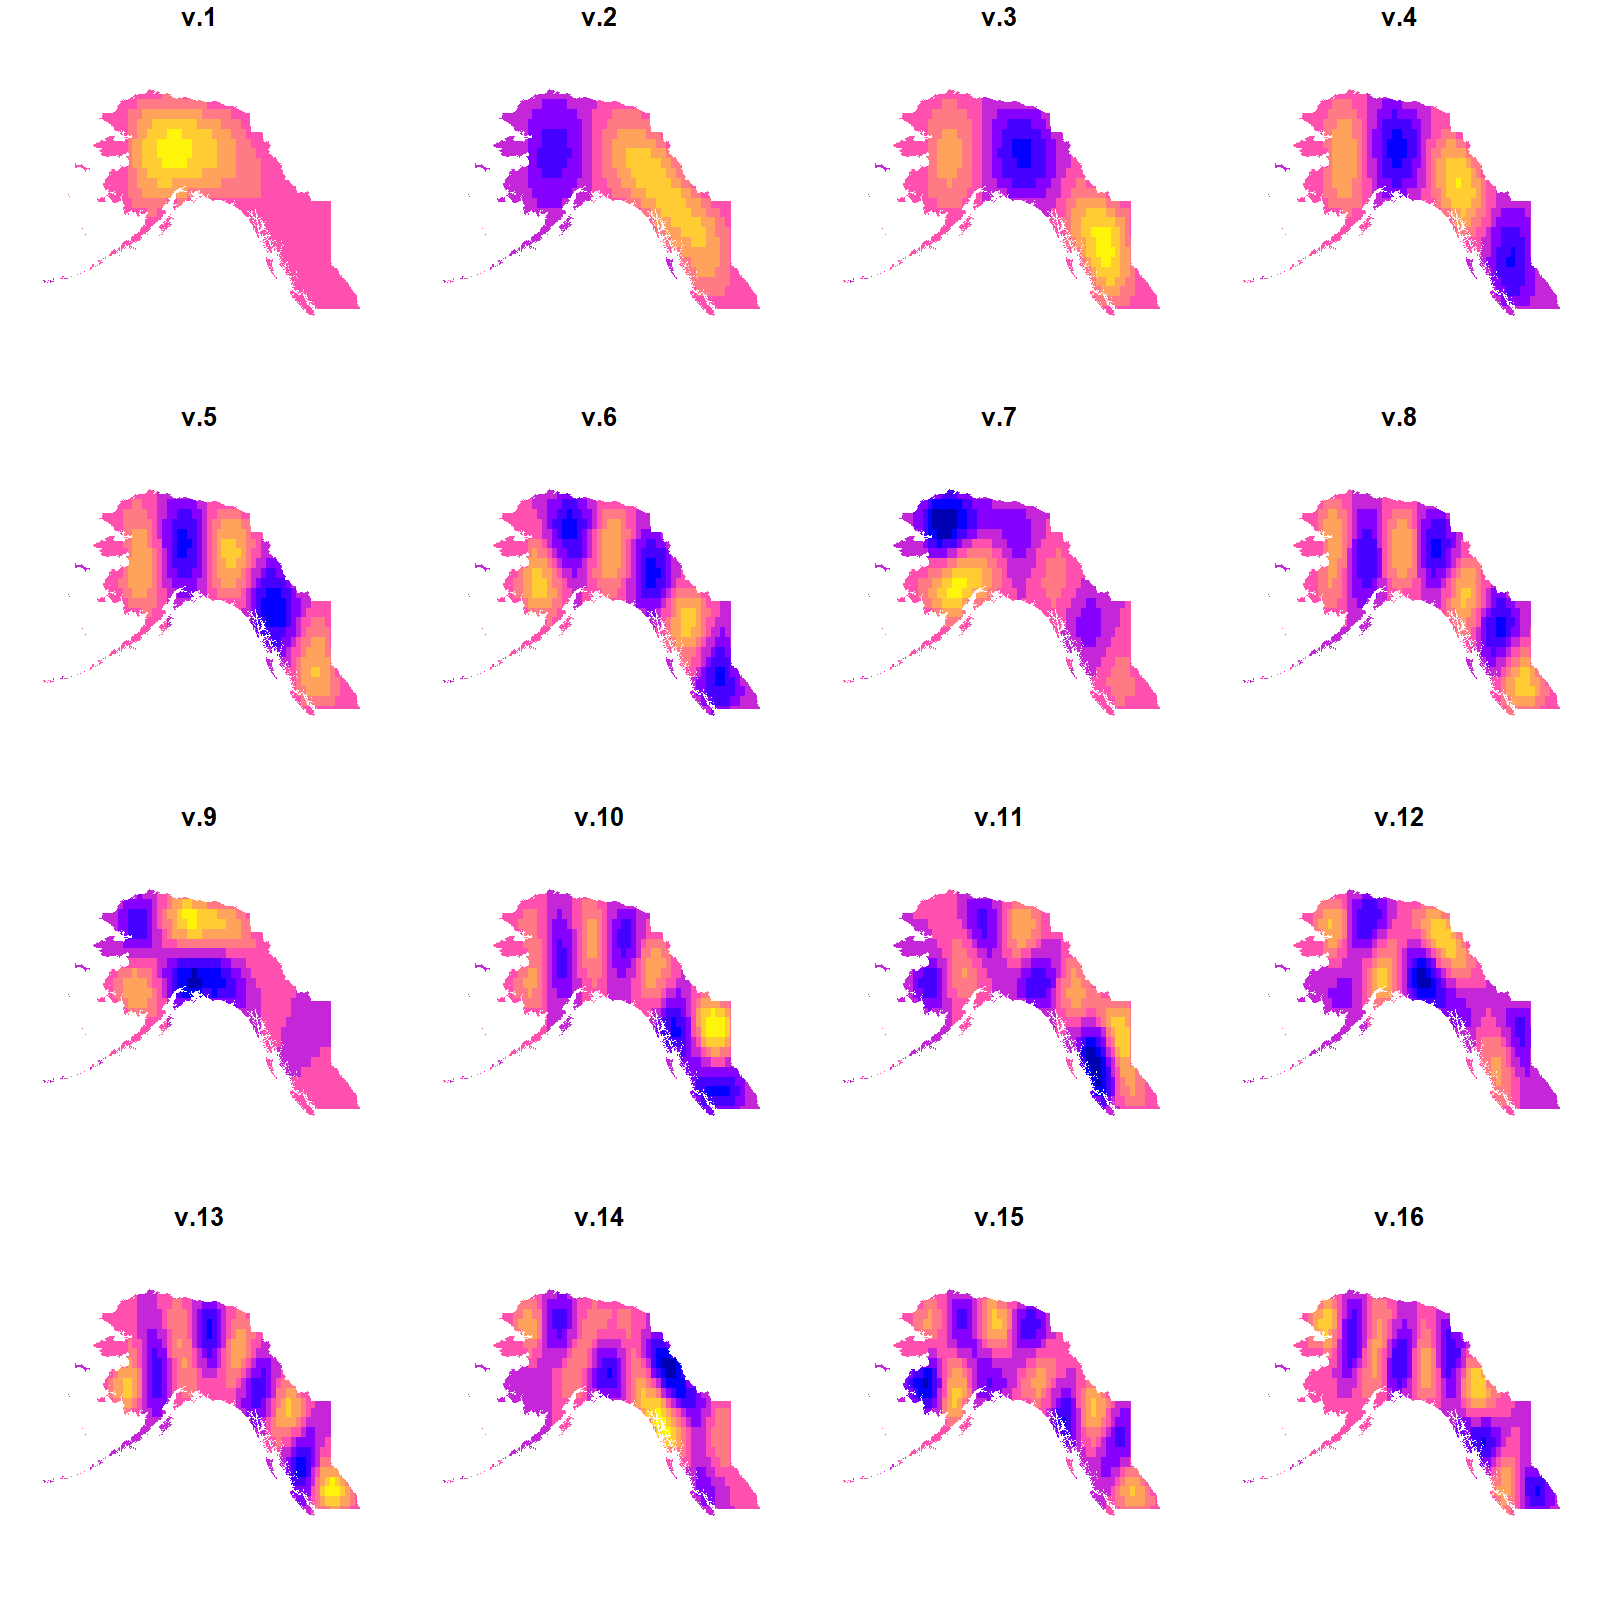
\includegraphics[width=5.5in]{Chap_5/Mapped_CAR_basis_functions.png}
    \label{fig:Chap5_CAR_basis_functions}
\end{figure}

Mapping estimated log-density using the CAR model (Fig \ref{fig:Chap5_CAR_densities}), confirms that it estimates high densities in southeast Alaska in agreement with the previous autoregressive methods (Fig. \ref{fig:Chap5_mapped_densities}).  Similarly, the estimated basis functions for the CAR (Fig \ref{fig:Chap5_CAR_basis_functions}) show patterns that are similar to those of the autoregressive methods (Fig. \ref{fig:Chap5_AR_basis_functions}), i.e., the first several basis functions represent broad spatial patterns followed by finer-scale variation for subsequent basis functions.    

\subsection{SPDE Method} \label{sec:Chap5_SPDE}

We next introduce an alternative stochastic partial different equation or \myindex{SPDE approach} to modelling a spatial variable measured at any set of locations in two dimensions \cite{bakka_spatial_2018,lindgren_explicit_2011}.  This approach has several noteworthy characteristics:
\begin{itemize}
    \item \textit{Customized resolution}:  the SPDE approach can be adapted to include a denser arrangement of random effects in some areas than others.  For example, in cluster sampling designs, it might be convenient to represent spatial variation at a high resolution near clustered sampling, while still using lower resolution elsewhere;

    \item \textit{Nonstationarity}:  it is relatively straightforward to include some types of nonstionarity, i.e., where the correlation rate varies as a function of covariates;

    \item \textit{Analytic and sparse precision matrix}:  similar to the CAR model, the SPDE method allows the precision matrix to be constructed directly for a 2D field, and the SPDE method also results in a precision matrix that is sparse.  This sparsity remains even when adding additional properties, e.g., an oscillatory covariance function \cite{lindgren_explicit_2011}; 

   \item \textit{Bounded or spherical domain}: we can easily adopt an irregular spatial domain.  For example, we can modify the model to avoid correlations that proceed across a boundary (e.g., over land when modelling correlations for a marine fish \cite{bakka_non-stationary_2019}) or include correlations arising on a sphere (e.g., when modelling correlations for an atmospheric measurement over the entire globe \cite{lindgren_explicit_2011});    
   
   \item \textit{Geometric anisotropy}:  finally, the SPDE method can be easily adapted to represent \myindex{geometric anisotropy}, defined as a correlation function that differs based on cardinal direction \cite{lindgren_explicit_2011,thorson_geostatistical_2015}.  This property is useful in ecological applications, e.g., when spatially correlated residuals (representing unmodeled exogenous or endogenous drivers) differ more greatly in one direction than another.
\end{itemize}
These characteristics could also be added to the CAR method shown previously, but the SPDE method provides a convenient user interface to do so.  

To introduce the SPDE approach, first recall that an autoregressive process for two locations \(s_1\) and \(s_2\) separated by distance \(d=|s_1-s_2|\) follows an  exponential correlation function, \( C_{exponential}(d) = e^{-\theta d} \), and that the precision matrix is zero for nonadjacent locations (see Eq. \ref{eq:Chap3_joint_precision}).  To generalize this for two dimensions, however, we have to define which locations are ``adjacent".  To do so, the SPDE method defines a \myindex{finite element analysis} (FEA) mesh.  This involves defining a set of triangles that cover the entire spatial domain, where every location is within exactly one triangle.  For example, the mesh for the bald eagles example has a higher density of triangles in southern British Columbia where samples are also dense (Fig. \ref{fig:Chap5_mesh}).  

\begin{figure}[!ht]
    \caption[Illustrating finite element mesh for bald eagle example]{The location of samples (blue circles in left panel) and the resulting finite element analysis mesh composed of triangles and with samples overlayed (right panel), showing the higher resolution (smaller triangles) arising in areas with many samples (blue points).}
    \centering
    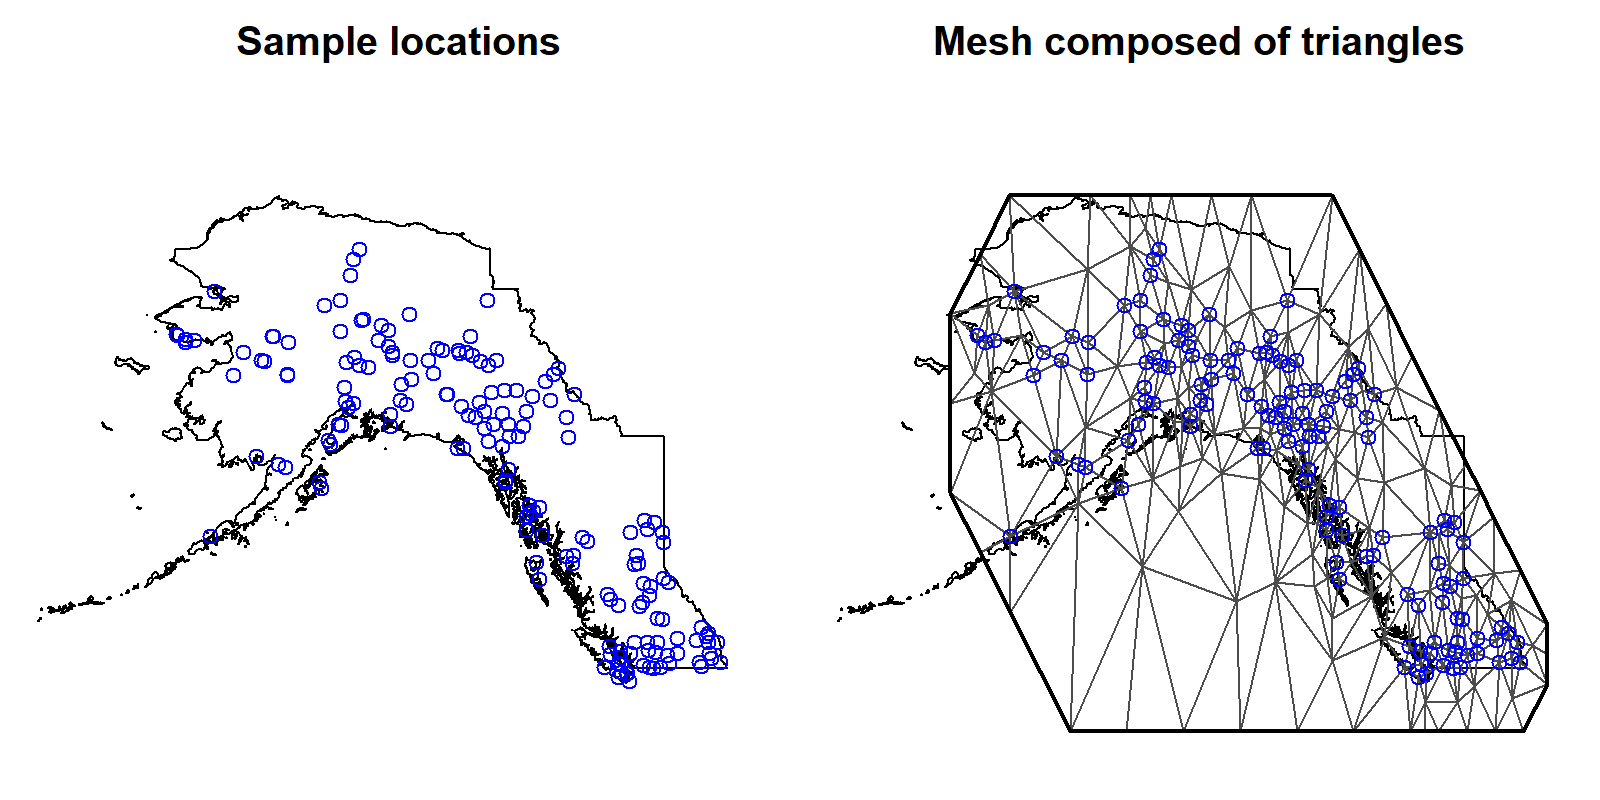
\includegraphics[width=5.5in]{Chap_5/SPDE_mesh.png}
    \label{fig:Chap5_mesh}
\end{figure}

This FEA mesh has several characteristics:
\begin{itemize}
    \item \textit{Vertices}: each triangle of the FEA mesh has three vertices, and the value of the spatial variable \(\omega_s\) at each of these vertices is treated as a random effect;
 
    \item \textit{Edges}:  similarly, each triangle of the mesh has three edges.  Two vertices are called \textit{adjacent} if and only if they are connected by a single edge.  
\end{itemize}
We also introduce the Matérn covariance function \cite{guttorp_studies_2006}:

\begin{equation} \label{eq:Chap5_matern_correlation_function}
    V_{matern}(d) = \frac{1}{\tau^2 2^{\nu-1} \Gamma(\nu)} (\kappa d)^{\nu} K_{\nu}(\kappa d)
\end{equation}
where \(\kappa\) is an estimated parameter representing the decorrelation rate (with units \(distance^{-1}\)), such that a high value of \(\kappa\) corresponds to a process where nearby locations have a low correlation, and \(\tau\) is the estimated parameter that controls the variance of the Matérn covariance function.  Finally, \(\nu\) is a parameter that is fixed a priori and controls how the smoothness of the Matérn covariance function, \(\Gamma(\nu)\) is the gamma function and \(K_{\nu}\) is a Bessel function.  This Matérn covariance function is useful in part because it reduces to the exponential covariance function when smoothness \(\nu = 0.5\), and approaches a Gaussian covariance function as smoothness \(\nu \rightarrow \infty\).  

Usefully, if we specify a smoothness that is intermediate between the exponential and Gaussian correlation functions (i.e., \(\nu = 1\) for a two-dimensional model), we can then approximate the precision matrix as:

\begin{equation} \label{eq:Chap5_SPDE_precision}
   \mathbf{Q}_{spde} = \tau^2 (\kappa^4 \mathbf{M}_0 + 2\kappa^2 \mathbf{M}_1 + \mathbf{M}_2)
\end{equation}
where \(\mathbf{M}_0\) is a diagonal matrix, \(\mathbf{M}_1\) is nonzero only vertices that are connected by an edge (i.e., the same sparsity as the adjacency matrix), and \(\mathbf{M}_2\) is nonzero only for vertices that are connected by two edges (i.e., the sparsity of the adjacency matrix squared).  In this example, \(\mathbf{M}_2\) still only has $<$9000 nonzero elements, such that 95\% of vertices are conditionally independent (Fig. \ref{fig:Chap5_SPDE_matrices}).  Using the Matérn correlation function (Eq. \ref{eq:Chap5_matern_correlation_function}) and \(\nu=1\), we also get simple expressions for the distance at approximately 10\% correlation (termed the \textit{geostatistical range}, \(\sqrt{8}/\kappa\)), and the variance as distance increases asymptotically (called the \textit{geostatistical sill} or pointwise variance, \(\frac{1}{4 \pi\tau^2 \kappa^2}\)).  These properties require us to fix \(\nu\) a priori, while only estimating \(\tau\) and \(\kappa\).  In general, we suspect that having a computationally efficient approach that is extensible (e.g., allows adding geometric anisotropy, covariate-based nonstationarity, or a customized domain) is more important than estimating \(\nu\) to bridge performance between the exponential and Gaussian correlation functions \cite{simpson_order_2012}. 


\begin{figure}[!ht]
    \caption[Sparse matrices generated for SPDE method in bald eagle example]{Depiction of the three sparse matrices used to assemble the precision matrix using the SPDE method, showing the number of non-zero elements in each.}
    \centering
    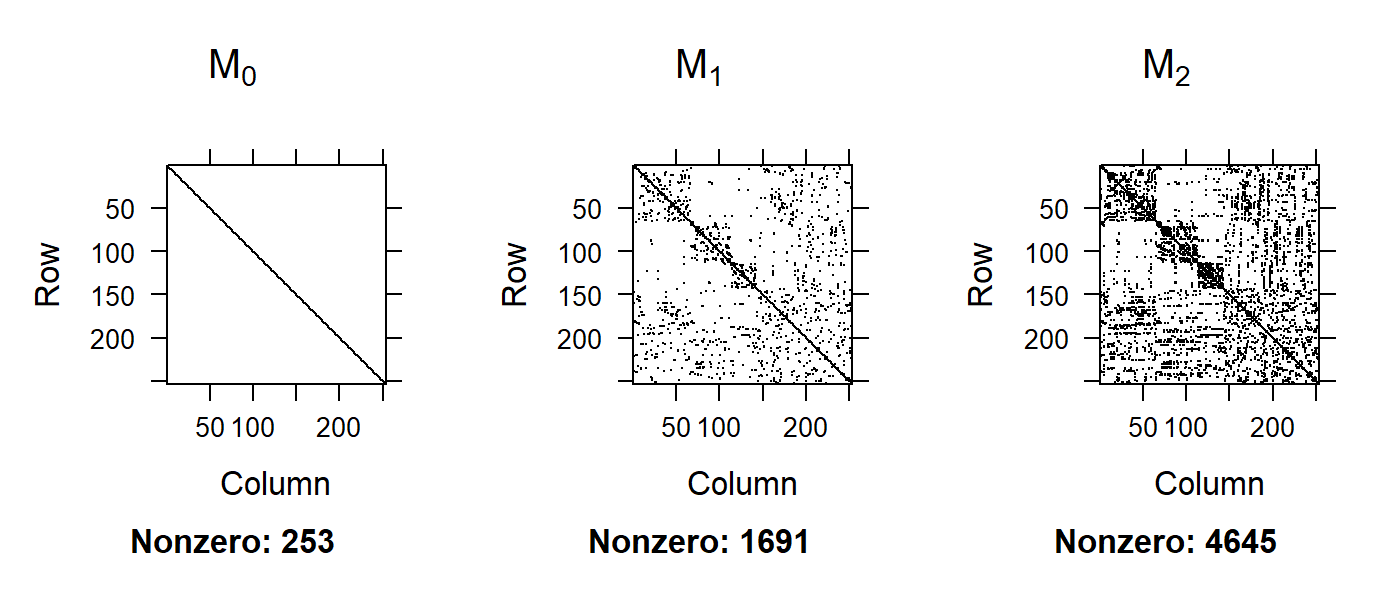
\includegraphics[width=5.5in]{Chap_5/SPDE_matrices.png}
    \label{fig:Chap5_SPDE_matrices}
\end{figure}

This SPDE method then allows the value of a spatial variable \(\omega_s\) at vertices \(s \in {1,2,...,S} \) to be computed as a multivariate normal distribution, \( \mathbf{\omega} \sim \mathrm{MVN}(\mathbf{0},\mathbf{Q}_{spde}^{-1}) \).  We then can interpolate the value \(\omega^*\) at any other locations as:

\begin{equation}
    \mathbf{\omega}^* = \mathbf{A \omega}
\end{equation}
where \(\mathbf{A}\) is a sparse matrix that represents bilinear interpolation.  Specifically, for any location \(g\) we identify the triangle of the finite-element mesh that contains it, identify the value \(\omega_s\) at its three vertices, and calculate \(\omega_g^*\) as a weighted average of these three values based on the distance between \(g\) and those three vertices.  The bilinear interpolation matrix \(\mathbf{A}\) represents this process by being nonzero for only three values in each row, with values representing weights used in that weighted average. 

\lstset{style=Rcode}
\lstinputlisting[language=R, label=code:Chap5-INLA, firstline=119, lastline=134, caption=R code to construct objects required for the SPDE method using the \colorbox{backcolour}{fmesher} package., captionpos=t]{Chap_5/SPDE.R}

Usefully, these matrices \(\mathbf{M}_0, \mathbf{M}_1, \mathbf{M}_2\), and \(\mathbf{A} \) can be computed automatically using the R-package \colorbox{backcolour}{fmesher} \cite{lindgren_fmesher_2023} (Code \ref{code:Chap5-INLA}).  This package provides simplified access to functions originally provided by R-package \colorbox{backcolour}{INLA} \cite{lindgren_continuous_2012}, although we will use package \colorbox{backcolour}{fmesher} to simplify software dependencies.  We will typically export these matrices to TMB and evaluate the probability of random effects using the \colorbox{backblue}{density::GMRF} function (Code \ref{code:Chap5-SPDE-in-TMB}), and therefore do not otherwise need to install the R-package \colorbox{backcolour}{INLA}.  In this case, we have defined a vector of random effects \colorbox{backblue}{omega\_s}, and we also show how to project from the vector at SPDE vertices to the vector \colorbox{backblue}{omega\_i} at all sample locations using projection matrix \colorbox{backblue}{A\_is} (constructed using function \colorbox{backcolour}{fmesher::fm\_evaluator} in Code \ref{code:Chap5-INLA} and then passed to TMB).  This workflow allows us to combine the SPDE approach with other customized model components.  However, we note that some models explored throughout the textbook can instead be fitted using the Integrated Nested Laplace Approximation \cite{rue_approximate_2009}, after which R-package INLA is named.  The details of this nested Laplace approximation are beyond our intended scope, but detailed comparison suggests that estimates using INLA or the default Laplace approximation in TMB are quite similar, while TMB allows more customized control over model configuration \cite{osgood-zimmerman_statistical_2023}.  

\lstset{style=TMBcode}
\lstinputlisting[language=c++, label=code:Chap5-SPDE-in-TMB, firstline=38, lastline=44, caption=TMB code used to evaluate the probability of a random effect using the SPDE method and also project from the vector of random effects at SPDE vertices to the vector of sample locations., captionpos=t]{Chap_5/SPDE.cpp}

We then fit the bald eagle dataset using this SPDE method, again interpolating densities to an evenly spaced grid to display results using a second projection matrix \(\tilde{\mathbf{A}}\) (labeled \colorbox{backcolour}{A\_gs} in Code \ref{code:Chap5-INLA}).  As expected, this shows the same spatial patterns in estimated log-densities as using the 2D autoregressive grid (Fig. \ref{fig:Chap5_mapped_densities_SPDE}) or the CAR model (Fig. \ref{fig:Chap5_CAR_densities}).  Similarly, we can calculate the covariance at the set of locations that we use for plotting.  The covariance at those locations is then \( \mathbf{\Sigma} = \tilde{\mathbf{A}} \mathbf{Q}_{spde}^{-1} \tilde{\mathbf{A}}^t \).  If we then calculate the basis functions implied by that covariance matrix, we again see that the dominant basis functions represent broad-scale spatial patterns (Fig. \ref{fig:Chap5_SPDE_basis_functions}), similar to the previous CAR and 2D autoregressive methods.  We therefore conclude that the SPDE method provides a convenient generalization of the 2D autoregressive process for unequally spaced locations.  

\begin{figure}[!ht]
    \caption[GLMM estimates of bald eagle densities using SPDE method]{Estimated summertime density of bald eagles using a GLMM and the SPDE method (see Fig. \ref{fig:Chap5_mapped_densities} for details).}
    \centering
    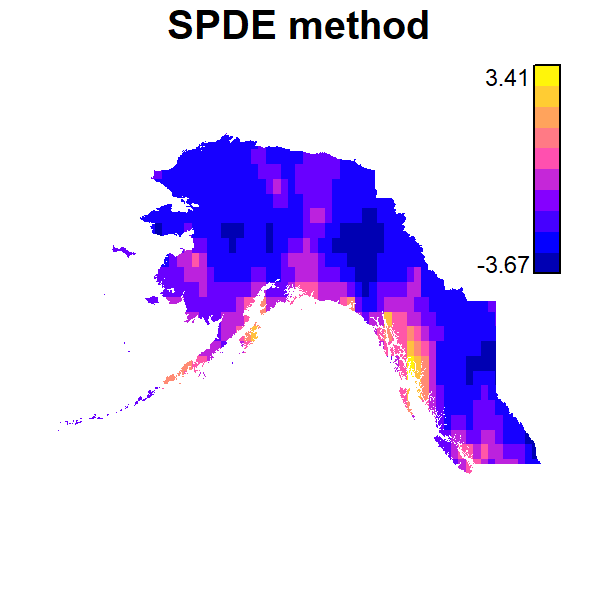
\includegraphics[width=3in]{Chap_5/Mapped_densities-SPDE.png}
    \label{fig:Chap5_mapped_densities_SPDE}
\end{figure}

\begin{figure}[!ht]
    \caption[Example of basis functions for SPDE method]{First 16 basis functions for the bald eagle species distribution model and the SPDE method (see Fig. \ref{fig:Chap5_AR_basis_functions} for details).}
    \centering
    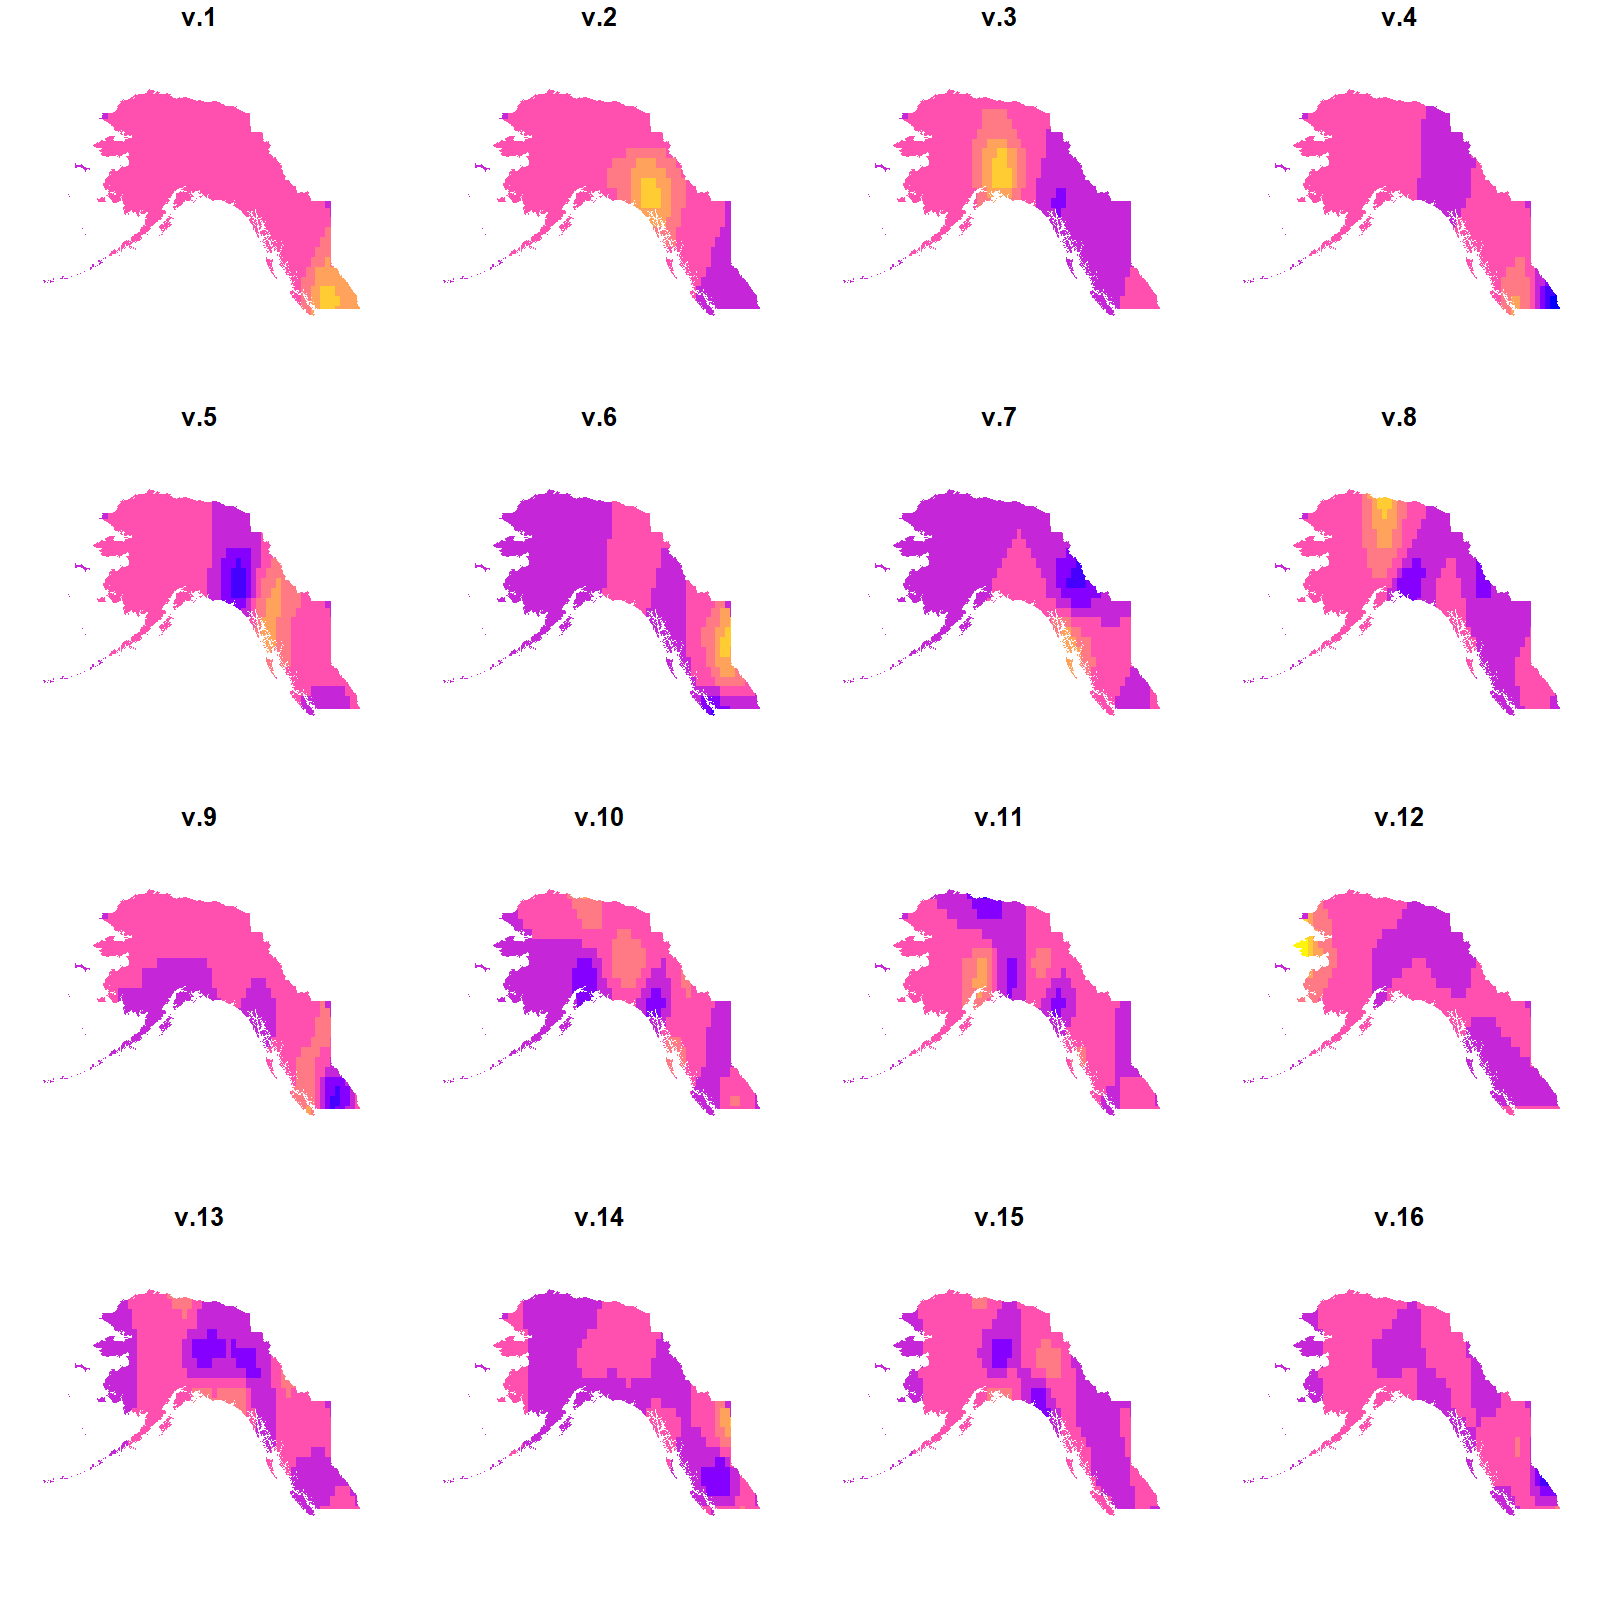
\includegraphics[width=5.5in]{Chap_5/Mapped_SPDE_basis_functions.png}
    \label{fig:Chap5_SPDE_basis_functions}
\end{figure}

\section{Chapter Summary}

In summary, we have showed that:
\begin{enumerate}
    \item Ecologists need a variety of approaches to identify spatially correlated residuals that remain when predicting population densities based on measured covariates, where these residuals arise from a variety of exogenous and endogenous mechanisms;

    \item Spatially correlated residuals can be addressed by using a basis-expansion of covariates, where basis expansion takes one or more covariates (e.g., elevation, temperature, location, etc.) and creates additional vectors that can more flexibly describe a nonlinear relationship between covariates and population response.  Two-dimensional basis expansion (i.e., for two spatial coordinates) then requires a tensor product of the basis-expansion for each individual covariate;
    
    \item Generalized Additive Models (GAMs) use splines for basis expansion, and penalize the coefficients for each spline towards zero.  This then shrinks the resulting function towards some smooth shape.  Similarly, generalized linear mixed models (GLMMs) using splines as covariates will use the log-determinant of the inner Hessian matrix as a penalty term, and with similar behavior to the penalty used by GAMs;
    
    \item We can define a two-dimensional (2D) distribution for a spatial variable by using a separable correlation function, i.e., the outer product of the correlation in each dimension individually. If each dimension uses a first-order autocorrelation with even spacing, then the resulting 2D grid has a precision matrix that is highly sparse;
    
    \item Alternatively, we can define a 2D distribution for an irregular grid using a conditional autoregressive process, or for any set of locations that approximates a Matérn correlation function by defining a finite element mesh and using the SPDE method.  All matrices involved in the SPDE approach can be produced easily using the fmesher package in R.  
\end{enumerate}

\section{Exercise}

Download elevation for samples and gridded locations in the bald eagle example (e.g., using package \colorbox{backcolour}{elevatr} used in Section \ref{sec:Chap5_tensor_spliens}).  Then, please adapt the code presented for either the CAR model or SPDE method, and add a quadratic or spline basis expansion of elevation to the linear predictor for that model.  After fitting, visualize the resulting response curve (e.g., adapting code from Section \ref{sec:Chap1_evaluating_model_fit} to use the \colorbox{backcolour}{marginaleffects} package).  Are the coefficients for this estimated effect of elevation statistically significant?

% \end{minipage}
% \end{center}